% \documentclass[preprint,12pt,authoryear]{elsarticle}
\documentclass[authoryear,preprint,review,12pt]{elsarticle}
\usepackage{amssymb}
\usepackage{amsmath}
\usepackage{caption}
\usepackage{subcaption}
\usepackage{multirow} 
\usepackage{bm}
\usepackage{lineno}
\usepackage{url} 
\journal{Engineering Structures}

\begin{document}

\begin{frontmatter}

\title{Surrogate Learning of Scour-critical Bridge Capacities and Uncertainty Quantification Considering Climate Scenarios}


\author[a]{Arian Qadir}
\author[b]{ZhiQiang Chen\corref{cor1}}
\affiliation[a]{organization={Graduate Student, Division of Natural and Built Environment, University of Missouri--Kansas City},%Department and Organization
            addressline={5100 Rockhill Rd.}, 
            city={Kansas City},
            postcode={64110}, 
            state={MO},
            country={USA}}
\affiliation[b]{organization={Professor, Division of Natural and Built Environment, University of Missouri--Kansas City},%Department and Organization
            addressline={5100 Rockhill Rd.}, 
            city={Kansas City},
            postcode={64110}, 
            state={MO},
            country={USA}}

\cortext[cor1]{Corresponding author; Email: chenzhiq@umkc.edu.}

%% Abstract
\begin{abstract}
Scour-critical bridges are among the most vulnerable transportation infrastructure systems, and their failure risk is expected to be increasingly uncertain due to climate change and climate-driven flood hazards. Traditional approaches often overlook the effects of such deep uncertainties and compute scour hazards assuming a single probabilistic distribution to analyze bridge capacity and collapse potential. This study develops a distribution-agnostic framework to predict the transverse capacities and quantify the uncertainties of scour-critical bridges. The major components include: (1) surrogate modeling of bridge capacities through learning from nonlinear pushover-based simulated data considering climate-scenario-based scour profiles, and (2) credal-set quantification of capacity uncertainties subject to climate-scenario scour profiles. The results reveal how variable uncertainties propagate through the nonlinear soil–foundation–structure bridge system when expressing the capacity tuple, including base shear, deck displacement, base moment, and column rotation. The resulting framework provides a novel analytics toolkit for climate-change and uncertainty-aware assessment of scour-critical bridge capacity, supporting engineers and transportation agencies in making resilient asset management decisions.
\end{abstract}




%%Research highlights
\begin{highlights}
\item A distribution-agnostic framework is proposed to assess scour-critical bridge capacity under climate-driven deep uncertainty.
\item Surrogate models are trained using nonlinear pushover simulations with climate-scenario-based scour inputs.
\item Credal-set uncertainty quantification is introduced to provide bounded predictions, ensuring objective capacity estimation.
\item Results support resilient decision-making for infrastructure adaptation and asset management under uncertain climate futures.
\end{highlights}


\begin{keyword}
Scour\sep
Bridge Capacity\sep
Surrogate Modeling\sep
Climate Scenario\sep
Credal Set\sep
Soil–foundation–structure Interaction\sep
\end{keyword}



\end{frontmatter}



\linenumbers






\section{Introduction}
Waterway bridge structures serve as critical nodes in transportation infrastructure, enabling vital socioeconomic connectivity. However, they are especially vulnerable to scour: the erosion of soil surrounding bridge foundations caused by flowing water. In the United States, over $600{,}000$ bridges span the nation's waterways, and an estimated $70\%$ were not originally designed to resist scour. Of these, approximately $21{,}000$ are classified as \textit{scour-critical} \citep{USGS2018}. Scour has historically been the leading cause of highway bridge failure, accounting for more than half of such collapses nationwide \citep{Sipson2019}. Looking ahead, climate change is projected to intensify scour risk in the $21^\text{st}$ century, as more frequent and severe riverine floods accelerate foundation erosion \citep{Cranston2022}. This convergence of inadequate original design, material aging, and worsening hydrologic hazards due to climate change highlights the need for predictive, risk-informed assessments of scour-critical bridges throughout their service life.

Developing reliable life-cycle performance quantification for scour-critical bridges is technically challenged by numerous factors. Among these, bridge scour as a hazard differs fundamentally from other natural and technological hazards (e.g., earthquakes and barge impacts). One key distinction lies in the uncertainties associated with scenario-based climate projections that are inherent in mainstream climate modeling methodologies, whether based on global climate models or downscaled regional models \citep{alizadeh2022advances,o2020achievements}. Researchers have long referred to such uncertainties as deep uncertainties (DUs), attributing them to hard-to-quantify or unknown factors such as long-term socioeconomic development, emission policy decisions, and technological change \citep{kandlikar2005representing}. The Intergovernmental Panel on Climate Change (IPCC) addresses these uncertainties by employing multiple climate scenario frameworks (e.g., Representative Concentration Pathways) that span optimistic to pessimistic emission trajectories. When adopted in hazard modeling (e.g., precipitation), these climate-driven DUs propagate through regional hydrological and hydraulic models (e.g., basin and riverine floods), and ultimately influence local scour profiles at waterway bridges.


Although researchers have acknowledged the complexity and implications of climate scenarios and deep uncertainties (DUs) for civil infrastructure design and management \citep{helmrich2022reconciling}, few studies have explicitly examined how these uncertainties affect bridge safety or design. Only in recent years have efforts emerged to integrate climate model outputs into scour risk assessments. For instance, Yang et al.\ linked downscaled climate data to bridge failure probabilities \citep{Yang2019}, and additional relevant studies are reviewed below. Nevertheless, a systematic treatment of scenario-driven uncertainty in bridge performance remains limited. Several investigations have incorporated climate-scenario information into scour or bridge risk modeling, yet significant gaps persist. Khelifa et al.\ quantified the influence of intensified flood regimes on scour-failure probabilities and economic losses; however, their framework employed deterministic structural limits and did not propagate climate-projection uncertainty into structural capacity metrics \citep{Khelifa2013}. Dikanski et al.\ explored the interaction between climate-model variability and asset-data uncertainty for a U.K. rail-bridge inventory, revealing that inadequate inventory data can overshadow climate uncertainty by an order of magnitude. Still, their analysis focused on the network level and did not address component-level performance or surrogate modeling \citep{Dikanski2018}. Liu et al.\ developed a network-level, risk-based adaptation framework for bridges facing climate-aggravated scour, but their approach relied on computationally expensive Monte Carlo simulations and was limited to discrete scenarios \citep{Liu2020}. Nasr et al.\ generated a national-scale map of Swedish catchments vulnerable to future pier scour but did not translate increased scour depths into structural safety margins \citep{Nasr2023}. Sasidharan et al.\ proposed a “warning-time-to-failure” index for climate-informed scour management while omitting probabilistic modeling of structural capacity or yield-based metrics \citep{Sasidharan2023}. Collectively, these studies highlight the need to model the systems-level behavior and scour risk considering climate scenarios; nonetheless, they do not focus on the intrinsic properties (namely, capacities) of scour-critical bridges. 

In Bridge Engineering practice, load rating has been a traditional approach for evaluating the vertical capacity of in-service bridges \citep{Cai2003,Scott2008,Gokce2011}. This procedure typically involves structural analysis based on LRFD-prescribed combinations of dead and live loads, hence defining the vertical capacity of bridges. For the assessment of waterway bridge collapse potential, the lateral capacity rating has primarily relied on nonlinear modal pushover analysis \citep{Alipour2013,Bignell2005}. These methods yield nonlinear pushover curves that are essential for characterizing lateral capacity under extreme transverse loads, such as those induced by seismic, hydraulic, or barge impact events. Capacity estimates are typically defined at the point of yielding, represented by the corresponding load and displacement values. However, few studies have addressed the variation in structural capacity as a function of varying scour depth. Moreover, no existing studies have explicitly incorporated climate scenario–induced scour uncertainties. A key technical barrier in addressing these gaps is the high computational cost associated with modeling complex nonlinear bridge systems under variable scour conditions.


Given the aforementioned research gaps, there is a compelling need to integrate modern data-driven modeling approaches for modeling and understanding lateral capacities of scour-critical bridges with the deep uncertainties inherent in climate scenarios. These machine learning (ML) methods, while distinct from traditional finite element or first-principles–based approaches, often remain dependent on simulation data generated through conventional techniques. However, once trained on such data, the resulting ML models, i.e. surrogates, can serve as computationally efficient predictive tools. Moreover, by directly mapping inputs (e.g., scour depth) to outputs (e.g., structural capacities), these models enable efficient quantification of predictive uncertainty—an essential capability when addressing scenario-based deep uncertainties central to this study.


This study proposes a novel modeling framework, which includes (1) surrogate learning of the structural capacities of scour-critical bridges under climate scenario–induced deep uncertainties and (2) quantification of climate-scenario-induced scour uncertainties without assuming a specific distribution of scour profiles. Statistically, the proposed framework is distribution-agnostic in nature. In summary, the paper presents the following key contributions:
\begin{enumerate}
    \item \textit{Surrogate Learning Framework for Scour Capacity.} A surrogate learning framework is developed to efficiently predict the structural capacity of scour-affected bridges using a library of nonlinear pushover analyses, enabling rapid capacity estimation without the need for repeated high-fidelity simulations.
    \item \textit{Capacity Tuple Definition.} A multi-dimensional capacity tuple is introduced to capture critical performance measures at yielding, including: (i) base shear, (ii) deck displacement, (iii) pile-cap moment, and (iv) pile-cap rotation—collectively characterizing both superstructure and substructure limit states.
    \item \textit{Climate-Induced Deep Uncertainty Quantification.} Deep uncertainties are incorporated via a credal-set approach, providing upper and lower bounds on capacity predictions across various climate scenario trajectories and yielding a robust envelope of predictive outcomes.
\end{enumerate}

In the following, this paper starts with a literature review of related efforts and techniques used in this work. Subsequently, it presents the proposed surrogate learning and uncertainty quantification framework. The numerical results given the select climate-scenario scour hazards and a representative bridge model are presented. The paper further discusses the implications, limitations, and directions for future research, followed by the conclusion. 

\section{Related Efforts and Techniques}
\subsection{Related Efforts}

Numerous studies have addressed the impact of variable scour profiles within fragility modeling frameworks. In some approaches, scour depth is treated as a conditional variable; in others, a fully probabilistic treatment is adopted, modeling scour as a hazard with an assigned distribution. Since scour not only acts as a primary hazard but also alters the boundary conditions at the foundation level, it is frequently analyzed in combination with other extrinsic natural hazards, resulting in multi-hazard assessment frameworks. Within this domain, several key findings have emerged:

\begin{itemize}
    \item \textit{Scour + Seismic.} Wang et al.\ \citep{Wang2014} showed that even moderate scour depths ($<$ 2\,m) can double the probability of column yielding during design-level earthquakes. Guo and Chen \citep{Guo2015} extended this work to a life-cycle framework, while Guo et al.\ \citep{Guo2016} developed time-dependent fragility functions that shift toward lower peak ground accelerations (PGAs) as scour severity increases. Parametric and copula-based approaches (e.g., Argyroudis and Mitoulis \citep{Argyroudis2021}) corroborate these findings across various bridge typologies.
    \item \textit{Scour + Barge Impact.} Kameshwar and Padgett \citep{Kameshwar2018} incorporated scour-dependent lateral support loss into vessel collision models, finding that collapse probability increases sharply once scour depth exceeds roughly 1.5 pier diameters. Fan et al.\ further integrated corrosion effects and nonlinear soil–pile interaction, revealing a shift in dominant failure mode from the superstructure to the pile foundation \citep{Fan2021}. \citet{guo2023probabilistic} developed impact fragility analysis to characterize bridge failure under barge collision and local scour hazards.
    
    \item \textit{Scour + Flood Debris / Flow.} Anisha et al.\ \citep{Anisha2022} jointly modeled debris impact, inundation pressure, and scour, concluding that a 1.5\,m scour depth increases flood-induced failure probability by approximately 80\%. Karriqi et al.\ \citep{Karriqi2024} investigated sequential loading scenarios (earthquake followed by flood-induced scour), observing moderate but systematic increases in system-level fragility.
\end{itemize}

Despite variations in modeling strategies, these studies share a common approach to probabilistically estimating structural collapse. For a generic structure, this begins by defining a displacement-based capacity measure: typically, the yielding displacement denoted $\Delta_y$, obtained via nonlinear pushover analysis. A corresponding response-demand quantity, $\Delta$, is then computed by simulating structural response under hazardous forces (e.g., from seismic or barge-impact loadings) characterized by an intensity measure $H$. The collapse event is then defined as the normalized demand $u = \Delta / \Delta_y$ exceeding a threshold value $u_t$, namely $u > u_t$. Through stochastic simulation that incorporates load and material uncertainties, researchers estimate the conditional probability of collapse, $P(u > u_t \mid H)$, namely collapse fragility. For conventional structures with fixed boundary conditions, $\Delta_y$ is treated as a constant property of the structure. However, in scour-critical bridges, $\Delta_y$ varies with scour depth, as scour alters the boundary conditions at the foundation level. Furthermore, it introduces ambiguity in selecting an appropriate threshold constant, $u_t$. 

To illustrate this concept, Figure~\ref{fig:figure1} presents three nonlinear pushover profiles corresponding to different scour conditions. The solid curve, with yielding capacity $(\Delta_{y0}, V_{y0})$, represents the non-scour case. The dashed curve with $(\Delta_{y1}, V_{y1})$ corresponds to a moderate scour scenario, and the dot-dashed curve with $(\Delta_{y2}, V_{y2})$ reflects a severe scour condition. If a constant capacity, such as $\Delta_{y0}$, is used to evaluate collapse potential across all scenarios, the resulting index $u = \Delta / \Delta_{y0}$ would misleadingly suggest equal vulnerability to collapse for the underlying bridge with the varying scour conditions. This highlights a fundamental limitation in using fixed capacity metrics under variable scour conditions. Moreover, as shown in Figure~\ref{fig:figure1}, both displacement and strength capacities ($\Delta_y$ and $V_y$) are reduced with increasing scour severity. Consequently, collapse limit states for scour-critical bridges must account for reductions in both strength and displacement capacities to reflect realistically the system capacity under scour-induced degradation.

\begin{figure}[htbp]
    \centering
    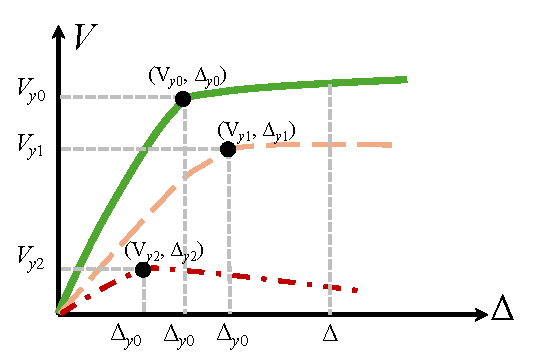
\includegraphics[width=0.6\linewidth]{Figures/Figure01.pdf}
    \caption{Illustration of representative nonlinear pushover curves for scour-critical bridge structures under varying scour profiles.}
    \label{fig:figure1}
\end{figure}

\subsection{Climate-scenario Uncertainty and Spatial Analogue}

Decision-making in hydraulic and infrastructure engineering under climate change is increasingly challenged by \textit{deep uncertainties} associated with various climate scenarios \citep{IPCC2022}. This condition is particularly acute in the context of projecting localized flood hazards, where uncertainty propagates across multiple modeling layers, from global climate models (GCMs) to regional downscaling, and more localized hydrological simulations \citep{Lafferty2023}.

Under such uncertainty, conventional risk-based planning methods that rely on probabilistic forecasts become insufficient. As emphasized by Lempert et al.\ \citep{Lempert2024}, deep uncertainty necessitates alternative strategies that explore a broad range of plausible futures rather than optimizing for a single forecast. In this context, \textit{Robust Decision Making (RDM)} and \textit{Dynamic Adaptive Policy Pathways (DAPP)} have emerged as leading frameworks.

One practical implementation of these strategies in hydrological risk assessment is the use of \textbf{spatial analogue}: the substitution of geographically distinct but hydrologically relevant locations to represent potential future conditions at a target site. This space-for-time reasoning is rooted in the ergodic hypothesis, which asserts that spatial ensembles governed by similar physical processes can approximate temporal evolution \citep{Sivapalan2011}. In hydrology, this principle supports the idea that rivers in disparate climate regimes today may serve as empirical analogues for the future behavior of a local watershed under climate change.


This analogue-based scenario selection offers key advantages: it anchors scenario construction in observed extremes, supports empirical stress-testing aligned with IPCC guidance \citep{IPCC2022}, and enables site-specific yet transferable hazard modeling. In this study, selected watersheds serve as proxies for future conditions, forming the empirical basis for generating synthetic but physically plausible flood and scour scenarios. Moreover, by bypassing reliance on predefined probabilistic distributions, the spatial-analogue approach directly supports a distribution-agnostic framework for modeling scour-critical bridge capacities under deep climate uncertainty.

\subsection{Surrogate Modeling Methods}
Data-driven surrogate models have emerged as efficient alternatives for simulating nonlinear structural responses under uncertainty. Among them, Support Vector Regression (SVR) and Gradient Boosting Regression (GBR) are widely used due to their complementary strengths in learning complex relationships from limited or structured data. SVR aims to find a function $f(\bm{x})$ that minimizes a regularized $\epsilon$-insensitive loss, promoting both model flatness and tolerance to small errors. This makes SVR particularly effective when training datasets are small or the underlying structural behavior is smooth. GBR, on the other hand, constructs an additive ensemble of shallow decision trees, where each successive tree fits the residuals of the previous one. This sequential learning strategy enables GBR to capture sharp nonlinear transitions and feature interactions effectively. Comparatively, toward generalization, SVR leverages kernel-based representations to generalize well in low-data regimes, while GBR achieves high predictive accuracy by exploiting structural hierarchies in unseen data. For formal mathematical formulations of SVR and GBR, readers are referred to \citep{Smola2004SVR,Friedman2001GBR}.

Many researchers adopted SVR and GBR as surrogate modeling techniques modeling structural behavior in Civil Structural and Infrastructure Engineering [e.g., \citep{xu2020surrogate,wang2022machine}]. Specifically, recent benchmarking studies, including Zhao et al.\ \citep{Zhao2023}, demonstrate that SVR and GBR consistently outperform linear models and often rival deep learning approaches, while requiring significantly less computational effort. These properties are especially advantageous in uncertainty quantification tasks, where repeated evaluation of surrogate models is necessary. In this study, SVR and GBR were selected as surrogate modeling techniques based on their proven performance in structural engineering applications. 

\subsection{Uncertainty Quantification Methods}
Modern machine learning and statistics provide several methods to estimate prediction uncertainty; representative ones include:
\begin{itemize}
    \item \textit{Bayesian Predictive Intervals:} Bayesian approaches (e.g., Gaussian processes) yield posterior distributions and credible intervals by treating model parameters as random variables \citep{Rasmussen2006}.
    
    \item \textit{Conformal Prediction:} Conformal methods produce intervals with finite sample coverage guarantees, assuming future data follow the same distribution as training \citet{Angelopoulos2021}
    
    \item \textit{Credal Sets:} Rather than a single distribution, a credal set represents a set of plausible probability measures for the output, capturing both aleatory and epistemic uncertainty \citep{Walley1991,Hofman2022}.
\end{itemize}

While Bayesian and conformal intervals perform well in many practical situations, they often underestimate uncertainty when facing distributional shifts or deep epistemic uncertainty. In this work, we adopt credal set methods to characterize uncertainties associated with bridge capacity prediction. This nonparametric distribution-agnostic approach yields a robust envelope that widens in regions of high epistemic uncertainty, as model disagreement increases \citep{Breiman1996}. % 

\section{Methodology}
\subsection{Overview}

Figure~\ref{fig:figure2} outlines the overall framework, which integrates three major components:
\begin{itemize}
    \item[1.] Scenario Selection, Scour Hazard, and FE Model Generation. This is a preparation stage that focuses on establishing the foundational inputs for simulation, including specific hydraulic flow scenarios and a suite of scour conditions generated using probabilistic sampling. The finite-element model of the bridge of interest is systematically modified for each sampled scour condition.

    \item[2.] Nonlinear Pushover Simulation and Capacity Extraction. This component executes nonlinear analyses for each scour case and extracts yield-level capacity responses. The outputs form a dataset for surrogate model training.

    \item[3.] Surrogate Modeling and Credal-Set Uncertainty Quantification (UQ). The final stage replaces computationally expensive simulations with lightweight machine learning models, enabling rapid capacity prediction and uncertainty quantification.
\end{itemize}

\begin{figure}[htbp]
    \centering
    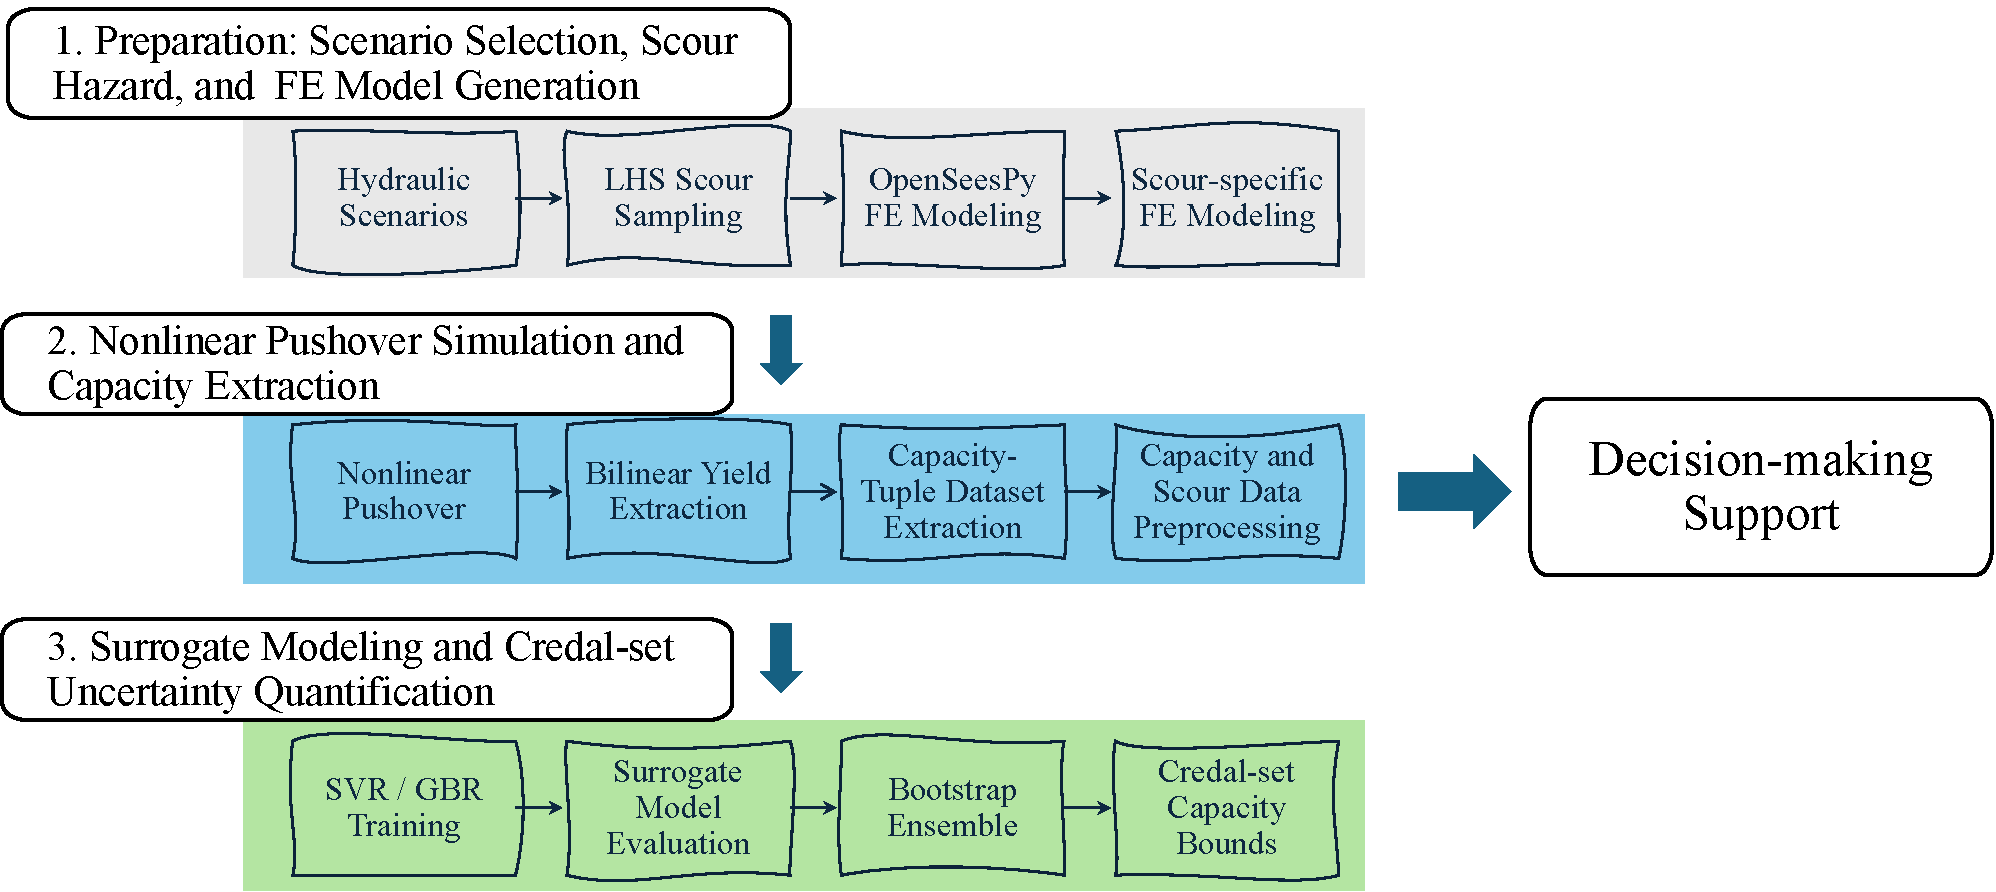
\includegraphics[width=0.8\linewidth]{Figures/Figure02.pdf}
    \caption{Proposed surrogate modeling and uncertainty quantification framework and methodological components.}
    \label{fig:figure2}
\end{figure}

Critical technical details and intermediate results from the climate-scenario-based scour analysis, FE modeling, and capacity value extraction are presented in the following subsections. Technical methods for surrogate modeling and credal-set uncertainty quantification are described subsequently, followed by major result interpretations. The workflow is implemented using Python, including OpenSeesPy \citep{OpenSeesPyDoc} for FE simulation and Scikit-learn \citep{scikit-learn} for machine learning and uncertainty quantification.

\subsection{Scenario Selection and Scour Hazard Calculation}

The specific design case involves a bridge spanning an imagined Midwestern river channel. Given the difficulty of downscaling peak flow velocities from global climate projections, the spatial-analogue concept is adopted in this work. Each scenario corresponds to a flooding event of increasing severity and is tied to a potential climate future near the year 2050, as structured by the SSP scenarios in IPCC AR6 \citep{IPCC2022}.

We identify two real-world rivers and one assumed worst-case as analogs to capture the range of plausible future extremes (Table~\ref{tab:combined_scenarios}):
\begin{itemize}
    \item \textit{Scenario 1 – Moderate (U = 2.9 m/s):} Based on average flood velocities reported for the \textit{Missouri River}, this case represents a baseline future in which climate change causes moderate increases in flow velocities \citep{modot2020tr202017}.
    
    \item \textit{Scenario 2 – High (U = 6.5 m/s):} Represents peak flood conditions in a more extreme but still physically observed context, based on field measurements from the \textit{Colorado River} during a major flood event \citep{Dawson2009}. This scenario reflects the increased intensity and flashiness expected in some AR6 pathways (e.g., SSP5-8.5).
    
    \item \textit{Scenario 3 – Extreme (U = 10 m/s):} A worst-case design flood velocity estimated for major Midwestern river systems under 500-year recurrence conditions. This provides an upper envelope for stress-testing structural safety and resilience.
\end{itemize}

To characterize long-term pier scour under variable hydraulic conditions, this study adopts the erosion framework from Briaud et al.\ \citep{Briaud1999}, widely used for cohesive soils and implemented in HEC-18. The adopted erosion rates $\dot{z}$, classified based on Briaud’s framework, are summarized in Table~\ref{tab:combined_scenarios}, corresponding to the selected scenarios and expected hydraulic conditions. It is noted that herein the notation $z$ is adopted for scour and erosion following \citet{Briaud1999}, which does not refer to the $z$ coordinate. Later, for surrogating modeling, the symbol $S_z$ is defined as a scour depth variable. 

\begin{table*}[htbp]
\caption{Scenario-Based Hydraulic Inputs and Scour Predictions (LHS, $N=1000$)}
\label{tab:combined_scenarios}
\centering
\small
\resizebox{\textwidth}{!}{%
\begin{tabular}{|c|c|l|c|c|c|c|}
\hline
\textit{Scenario} & $U$ (m/s) & \textit{Analog River (Flow Description)} & $\dot{z}$ (mm/h) & $\mu_{\text{scour}}$ (m) & $\sigma$ (m) & 95$^{\text{th}}$-Perc (m) \\
\hline
1 & 2.9 & Missouri River (avg. flood) & 100 & 3.56 & 1.70 & 6.80 \\
2 & 6.5 & Colorado River (2009 peak) & 500 & 9.13 & 4.26 & 17.16 \\
3 & 10.0 & Midwestern extreme (500-yr design flood) & 1000 & 14.10 & 6.74 & 26.30 \\
\hline
\end{tabular}%
}
\end{table*}

First, the maximum hydraulic shear stress $\tau_{\text{max}}$ is defined as a function of upstream velocity $U$, water density $\rho_w$, and Reynolds number $Re$, computed as:

\begin{equation}
Re = \frac{U d_p}{\gamma}
\label{eq:reynolds}
\end{equation}
where $d_p$ is the pier diameter and $\gamma$ is the kinematic viscosity. The shear stress $\tau_{\text{max}}$ is then given by the semi-empirical relation:
\begin{equation}
\tau_{\text{max}} = 0.094 \cdot \rho_w \cdot U^2 \left[ \frac{1}{\log_{10}(Re)} - 1 \right]
\label{eq:shear}
\end{equation}

The maximum scour depth under clear-water conditions is expressed as:
\begin{equation}
z_{\text{max}} = 0.18 \cdot Re^{0.635}
\label{eq:zmax}
\end{equation}
This expression is derived from regression analysis of controlled tests conducted in cohesive soils \citep{Gudavalli1998}.

The equilibrium scour time $t_{\text{eq}}$ is modeled as a duration-based erosion process that scales with time $t$, flow velocity $U$, and initial scour rate $\dot{z}$:
\begin{equation}
t_{\text{eq}} = 73 \cdot t^{0.126} \cdot U^{1.706} \cdot \dot{z}^{-0.2}
\label{eq:teq}
\end{equation}

From this, the projected scour depth after 50 years, denoted $z_{50}$, is estimated by:
\begin{equation}
z_{50} = \frac{t_{\text{eq}}}{1 + t_{\text{eq}}} z_{\text{max}}
\label{eq:z50}
\end{equation}

To capture uncertainty in long-term scour development due to stochastic variability in material properties and hydraulic conditions, a lognormal model is used for the final scour depth. Given a standard normal variate $\epsilon \sim \mathcal{N}(0,1)$, the final scour depth is computed as:
\begin{equation}
z_{50}^{\text{final}} = \frac{e^{-0.085 z_{50}} \cdot e^{0.407 \epsilon}}{1000}
\label{eq:zfinal}
\end{equation}
where the denominator converts millimeters to meters. This probabilistic formulation aligns with previous risk-informed studies on scour and bridge resilience \citep{Alipour2013,Briaud2010}.

To approximate the distribution of introduced random variables, the Latin Hypercube Sampling (LHS) method is adopted. The scour-depth samples under the three different river flow conditions (Table~\ref{tab:combined_scenarios}) are simulated separately. For each scenario, the script generates 1,000 samples by converting flow velocity into estimated scour depth. It accounts for uncertainty in both hydraulic forces and soil erosion characteristics. Figure~\ref{fig:figure3a} and~\ref{fig:figure3b} illustrate the resulting distributions, including histogram plots, lognormal fits denoted by $f_{S_z}(z)$, and the fitted exceedance probability curves representing the hazard function: $P_{S_z}(Z > z) = 1 - \int_\infty^{z} f_{S_z}(z') \, \mathrm{d}z'$.

\begin{figure}[htbp]
    \centering
    \begin{subfigure}[b]{0.48\textwidth}
        \centering
        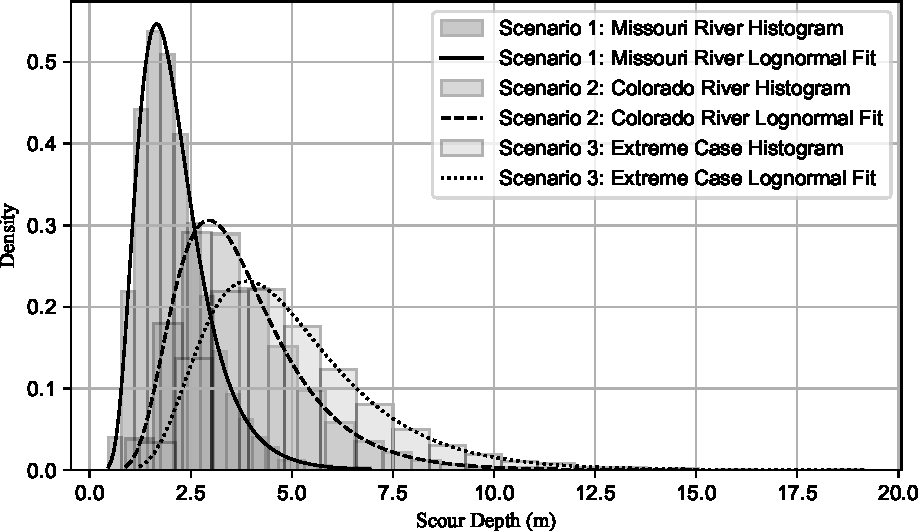
\includegraphics[width=\linewidth]{Figures/Figure03a.pdf}
        \caption{}
        \label{fig:figure3a}
    \end{subfigure}
    \hfill
    \begin{subfigure}[b]{0.48\textwidth}
        \centering
        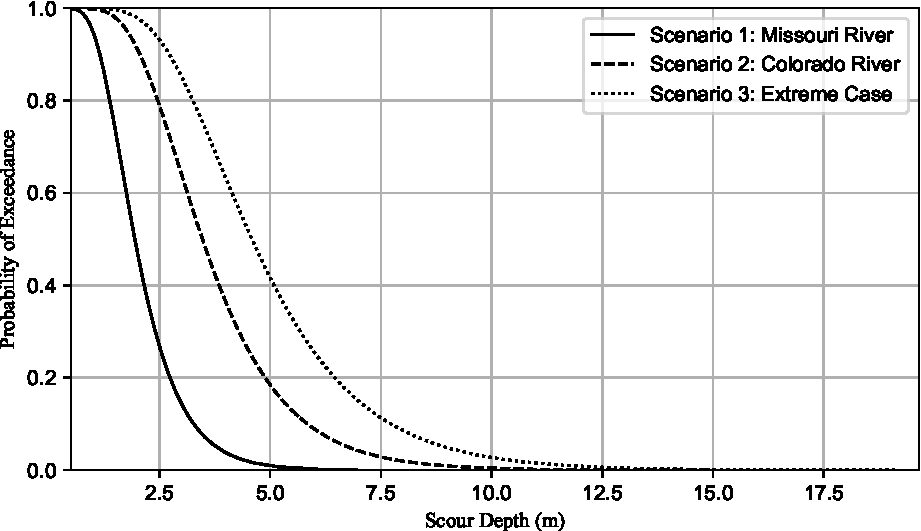
\includegraphics[width=\linewidth]{Figures/Figure03b.pdf}
        \caption{}
        \label{fig:figure3b}
    \end{subfigure}
    \caption{(a) Histogram distributions and lognormal fits for simulated climate scenario-based scour depth data. (b) Fitted hazard curves for cumulative distribution of simulated climate scenario-based scour depth data.}
    \label{fig:figure3}
\end{figure}

\subsection{Finite-Element Modeling}

As reviewed previously, many scour-critical bridge models have been developed in the literature. The framework proposed in this work is adaptable to any waterway bridge model, provided that climate-sensitive scour hazards are of interest. The bridge model adopted here is based on the one developed in \citet{Atak2014}, originally implemented using the OpenSees framework with the TCL language. In this study, the model is re-implemented in Python using the OpenSeesPy library. Figure~\ref{fig:figure4a} illustrates the transverse elevation of the bridge structure, and Figure~\ref{fig:figure4b} provides details of the primary elements developed in the OpenSeesPy environment.

\begin{figure}[htbp]
    \centering
    \begin{subfigure}[b]{0.8\textwidth}
        \centering
        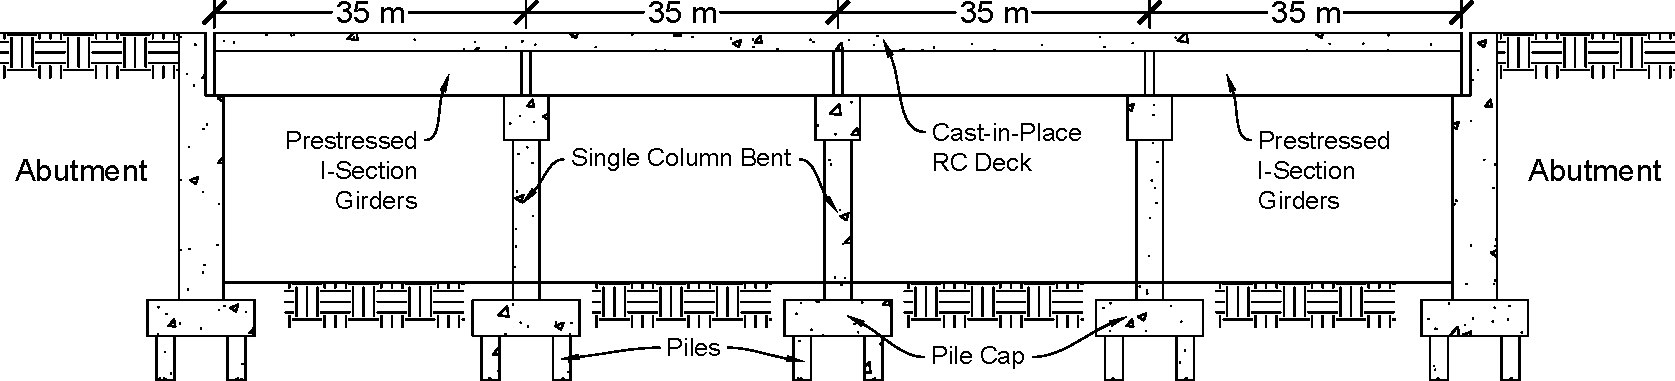
\includegraphics[width=\linewidth]{Figures/Figure04a.pdf}
        \caption{}
        \label{fig:figure4a}
    \end{subfigure}
    \begin{subfigure}[b]{0.8\textwidth}
        \centering
        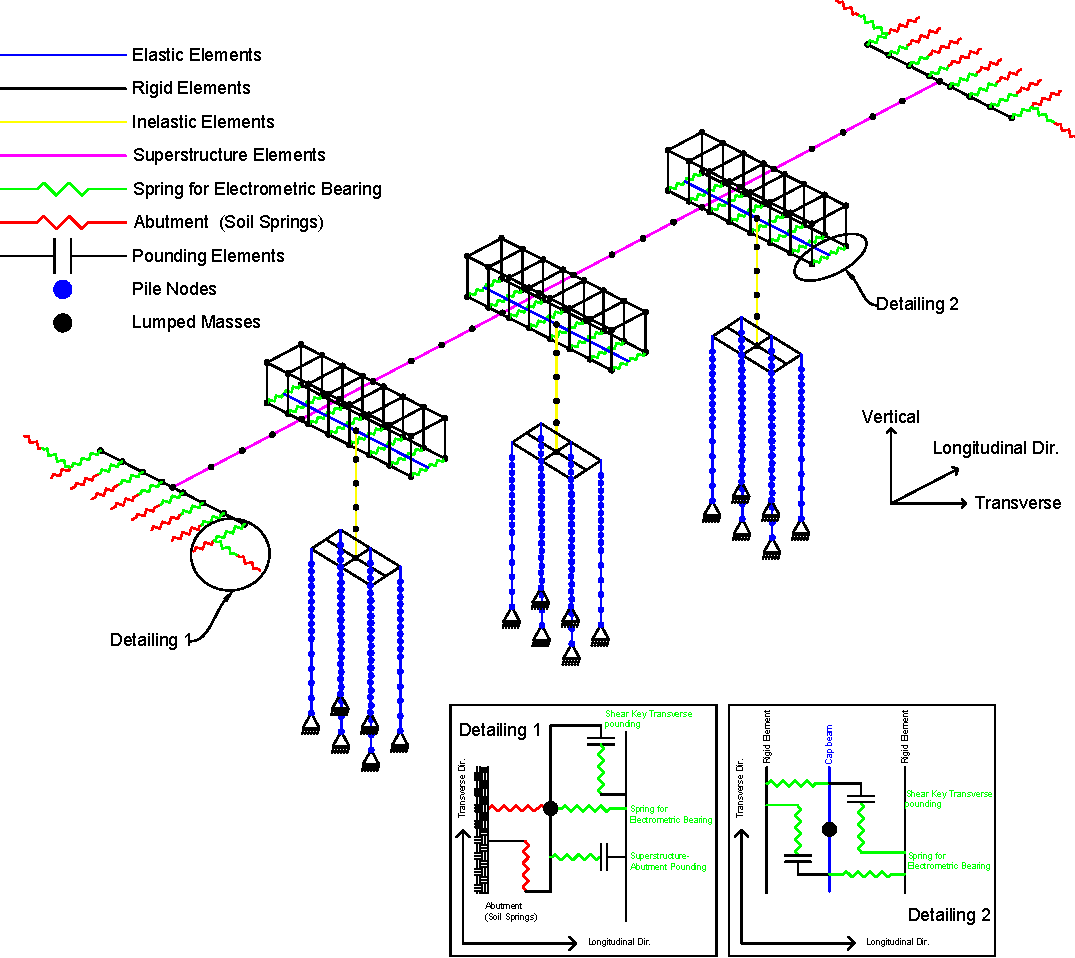
\includegraphics[width=\linewidth]{Figures/Figure04b.pdf}
        \caption{}
        \label{fig:figure4b}
    \end{subfigure}
    \caption{(a) Elevation view of the bridge structure. (b) The finite-element model with key nonlinear elements.}
    \label{fig:figure4}
\end{figure}

The modeled bridge represents a typical Midwestern U.S. bridge: a four-span, non-skewed prestressed concrete structure, with each span measuring 35 meters and a total deck width of 12 meters. The superstructure consists of I-girders supporting a cast-in-place concrete deck, resting on elastomeric bearings over reinforced concrete piers and pile group foundations embedded in layered soil.

The piers are modeled using nonlinear beam-column elements with fiber sections to accurately capture flexural behavior, confinement, and post-yield response. Each pier column is divided into five integration points, providing a detailed curvature distribution. The \texttt{Concrete01} material is used for both unconfined and confined concrete zones, while \texttt{Steel02} is adopted for reinforcing steel, with cyclic hardening parameters $R_0 = 15.0$, $c_{R1} = 0.9$, and $c_{R2} = 0.2$. Shear and torsional effects are captured using Aggregator sections.

Soil–structure interaction is modeled through nonlinear \texttt{zeroLength} springs at the pile–soil interface, simulating $p$–$y$ (lateral), $t$–$z$ (vertical), and $q$–$z$ (tip) behaviors following FHWA HEC-18 recommendations. These springs use the \texttt{PySimple1} material definition and are depth-dependent. Springs above the scour depth are deactivated to simulate soil loss, thereby reducing lateral and axial stiffness.

To reflect scour-induced soil loss, springs are progressively removed as scour depth increases. While material property uncertainties are included, they are intentionally minimized so that scour remains the dominant source of variability. Specifically, concrete compressive strength $f'_c$ is modeled as a normal distribution with a mean of 27.0 MPa and a standard deviation of 1.0 MPa. Steel yield strength $f_y$ is modeled using a lognormal distribution with a mean of 420.0 MPa and a standard deviation of 4.2 MPa.

Latin Hypercube Sampling (LHS) is employed with 1,000 samples per scenario (three scenarios in total), resulting in 3,000 simulations. This sampling approach robustly approximates the probabilistic scour hazard while keeping material variability constrained \citep{Hwang2000}. Figures~\ref{fig:figure5a} and \ref{fig:figure5b} depict the resulting histograms based on the sampled values for concrete and reinforcing steel strength, respectively.

\begin{figure}[htbp]
    \centering
    \begin{subfigure}[b]{0.48\textwidth}
        \centering
        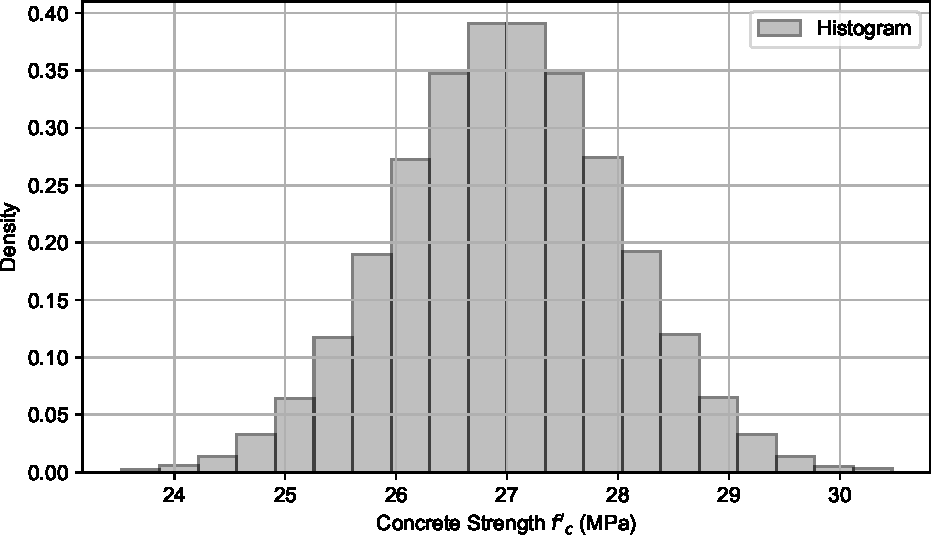
\includegraphics[width=\linewidth]{Figures/Figure05a.pdf}
        \caption{}
        \label{fig:figure5a}
    \end{subfigure}
    \hfill
    \begin{subfigure}[b]{0.48\textwidth}
        \centering
        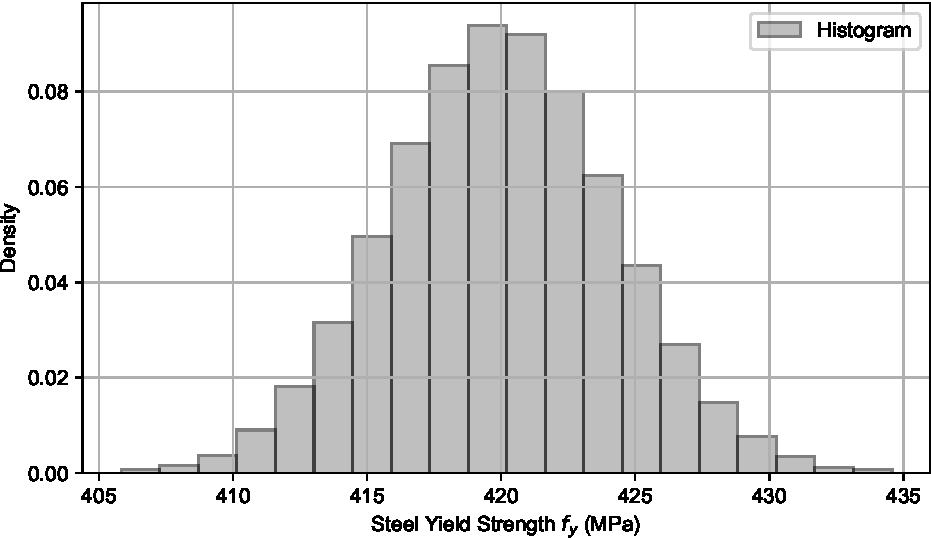
\includegraphics[width=\linewidth]{Figures/Figure05b.pdf}
        \caption{}
        \label{fig:figure5b}
    \end{subfigure}
    \caption{(a) Histogram of concrete compressive strength $f'_c$ (MPa). (b) Histogram of steel yield strength $f_y$ (MPa).}
    \label{fig:figure5}
\end{figure}

\subsection{FE Simulation and Capacity Extraction}

Pushover analyses were conducted for each simulation, tracking the force-displacement response at the top of the piers. A total of 3,000 nonlinear pushover simulations were performed, corresponding to Latin Hypercube Sampling (LHS)–generated scour cases across three hydraulic scenarios. For each scour case, the OpenSeesPy model was regenerated to reflect the corresponding scour depth by deactivating \texttt{zeroLength} soil springs (representing $p$–$y$, $t$–$z$, and $q$–$z$ behaviors) located above the scour level.

After applying and equilibrating gravity loads, a displacement-controlled pushover analysis was performed in the longitudinal direction (DOF = 2) at the deck level, targeting a maximum lateral drift of 5\% of the column height. A fallback strategy was implemented to ensure convergence, adaptively switching among Newton–EnergyIncr, Broyden, NewtonLineSearch, and Krylov-based solvers. Each simulation recorded top-node displacements, column rotations, base shears, and moments. The key structural responses at yielding were extracted and organized into a four-dimensional capacity tuple:

\begin{itemize}
    \item \textit{Yield Displacement} ($\Delta_y$): The horizontal displacement at the bilinear yield point, obtained from curve fitting.
    \item \textit{Yield Base Shear} ($V_y$): The lateral force corresponding to $\Delta_y$.
    \item \textit{Yield Moment} ($M_x$): The bending moment recorded at the base of the critical columns at yield.
    \item \textit{Yield Rotation} ($\theta_x$): The rotational deformation at yielding, computed from column displacement profiles.
\end{itemize}

This set of yield capacities $(\Delta_y,\ V_y,\ M_x,\ \theta_x)$ captures essential limit-state behaviors and supports cross-scenario performance comparisons. Each pushover response ($f$ vs.\ $d$) was smoothed and fitted using a segmented bilinear function:
\begin{equation}
\hat{f}(d) = 
\begin{cases}
    k_1 \cdot d, & d < d_y \\
    k_2 \cdot d + (k_1 - k_2) \cdot d_y, & d \geq d_y
\end{cases}
\label{eq:bilinear_fit}
\end{equation}

A profile-fitting algorithm (see Listing 1) minimized the squared residuals between the simulation output $f_i$ and the predicted values $\hat{f}(d_i)$:
\begin{equation}
J(k_1, k_2, d_y) = \sum_{i=1}^{N} \left[ f_i - \hat{f}(d_i;\,k_1, k_2, d_y) \right]^2
\label{eq:residual}
\end{equation}

The optimal yield displacement $d_y$ was selected by sweeping over a grid of candidate breakpoints. For each $d_y$, the best-fit values of $k_1$ and $k_2$ were computed using closed-form expressions:
\begin{equation}
k_1 = \max \left\{ 0, \frac{\sum_{i \in I_1} d_i f_i}{\sum_{i \in I_1} d_i^2} \right\}, \quad
k_2 = \frac{\sum_{i \in I_2} (d_i - d_y)(f_i - k_1 d_y)}{\sum_{i \in I_2} (d_i - d_y)^2}
\label{eq:k1_k2}
\end{equation}

Figure~\ref{fig:figure6} shows an example of bilinear fitting for one simulated scour depth. The yielding base shear and the corresponding deck-level displacement are extracted from this fit.

\begin{figure}[htbp]
    \centering
    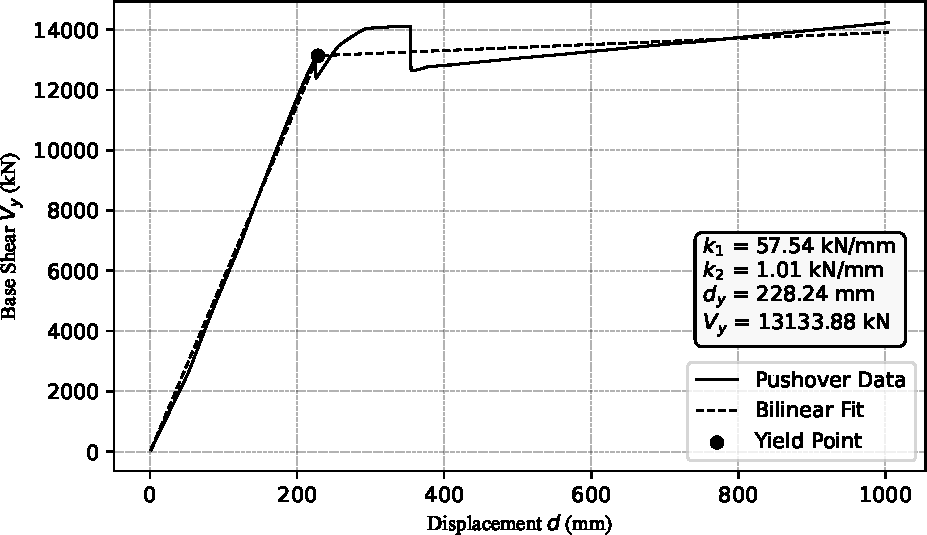
\includegraphics[width=0.6\linewidth]{Figures/Figure06.pdf}
    \caption{Illustration of capacity-tuple extraction using bilinear pushover curve fitting to extract $\Delta_y$ and $V_y$ at a scour depth of $7.347$ m.}
    \label{fig:figure6}
\end{figure}

Figure~\ref{fig:figure7} presents histogram plots for the extracted capacity values of all 3,000 simulations, combining the results from all climate scenarios: (a) $V_y$, (b) $M_x$, (c) $\Delta_y$, and (d) $\theta_x$. A key observation is that the resulting distributions deviate significantly from common parametric forms—exhibiting both skewness and multimodality. This indicates that fitting these distributions to standard probability models (e.g., normal or lognormal) is not meaningful, thereby reinforcing the need for nonparametric uncertainty quantification methods.

\begin{figure}[htbp]
    \centering
     \begin{subfigure}[b]{0.48\textwidth}
        \centering
        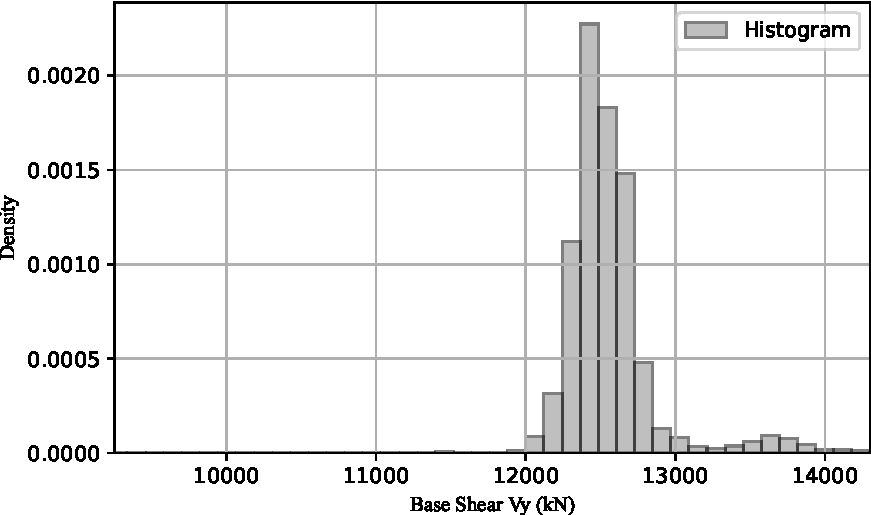
\includegraphics[width=\linewidth]{Figures/Figure07a.pdf}
        \caption{}
        \label{fig:figure7a}
    \end{subfigure}
    \hfill
     \begin{subfigure}[b]{0.48\textwidth}
        \centering
        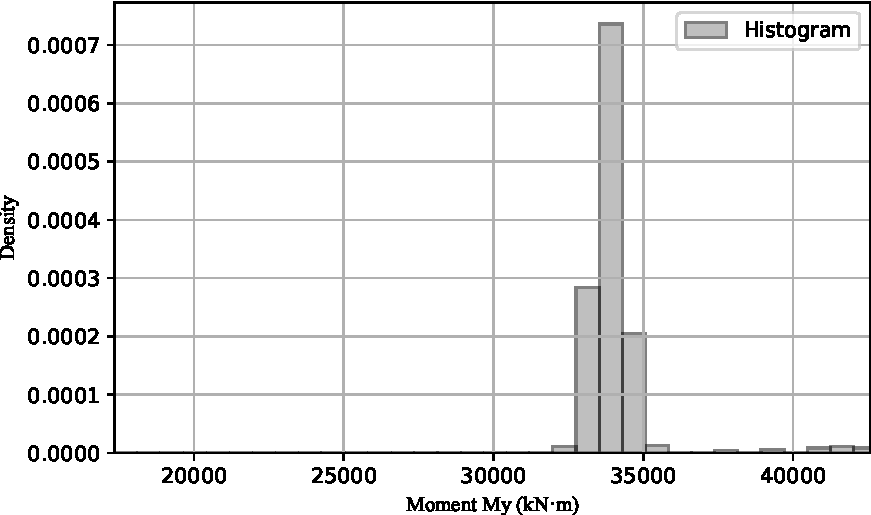
\includegraphics[width=\linewidth]{Figures/Figure07b.pdf}
        \caption{}
        \label{fig:figure7b}
    \end{subfigure}
    \hfill
     \begin{subfigure}[b]{0.48\textwidth}
        \centering
        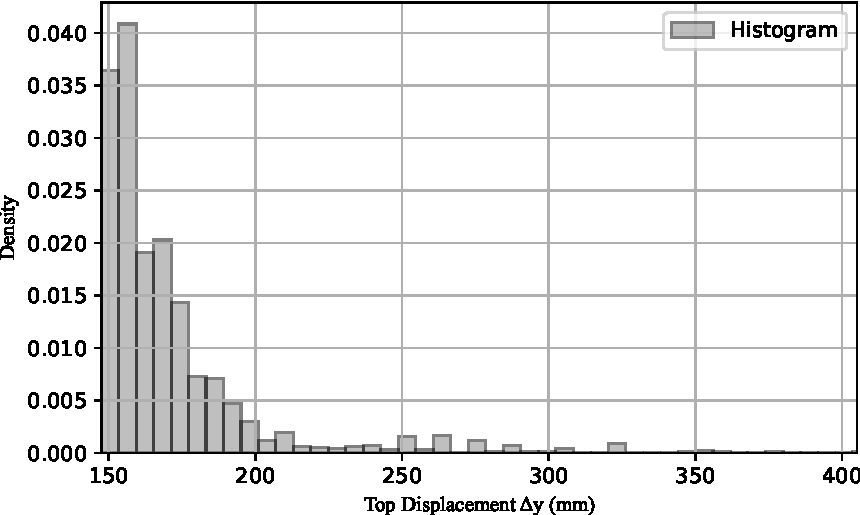
\includegraphics[width=\linewidth]{Figures/Figure07c.pdf}
        \caption{}
        \label{fig:figure7c}
    \end{subfigure}
    \hfill
     \begin{subfigure}[b]{0.48\textwidth}
        \centering
        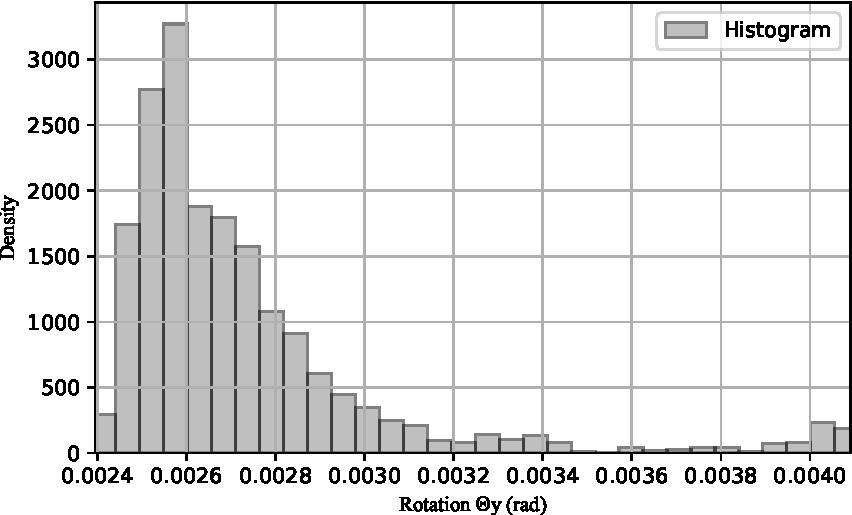
\includegraphics[width=\linewidth]{Figures/Figure07d.pdf}
        \caption{}
        \label{fig:figure7d}
    \end{subfigure}
    \caption{Resulting histogram plots for the bridge capacity tuple: (a) $V_y$, (b) $M_x$, (c) $\Delta_y$, and (d) $\theta_x$.}
    \label{fig:figure7}
\end{figure}

\subsection{Surrogate Modeling}
This study develops data-driven surrogate models to predict structural capacity measures directly from scour depth input. The goal is to replace computationally intensive finite-element simulations with lightweight predictive models mapping scour depth ($S_z$) to the four components of the capacity tuple:

\begin{equation}
S_z \xrightarrow{\text{Predict}} \Delta_y,\ V_y,\ M_x,\ \theta_x
\label{eq:sz_to_capacity}
\end{equation}
where $\Delta_y$ is the lateral displacement at yielding, $V_y$ is the base shear, $M_x$ is the flexural moment, and $\theta_x$ is the rotational deformation at yield. These surrogate models are trained using output from nonlinear pushover simulations, where each data point links a specific scour condition to a corresponding capacity tuple.

To enrich the input space and improve the model’s ability to approximate nonlinear patterns, we engineer features based on $S_z$: $S_z^2$, $S_z^3$, $\log(S_z)$, $1/S_z$, and $\sqrt{S_z}$. These transformations help the model capture both polynomial and asymptotic trends in capacity loss under increasing scour conditions.

Before model training, data were cleaned to remove incomplete or unstable simulations. An outlier filtering step was applied within scour-depth bins using the interquartile range (IQR) method: points lying outside $[\text{Q1} - 1.5 \times \text{IQR},\ \text{Q3} + 1.5 \times \text{IQR}]$ were discarded \citep{tukey1977exploratory}. This localized filtering prevented heavily scoured samples from distorting the statistical characterization of lightly scoured cases, and vice versa.



\subsubsection{Support Vector Regression (SVR).} 
Support Vector Regression (SVR) is a kernel-based learning algorithm that approximates a nonlinear function mapping input features to target responses. It projects the input vector $\bm{x}$ into a high-dimensional space using a kernel function (here, the Radial Basis Function or RBF kernel) and finds a function that fits the training data while ignoring small errors within a specified tolerance band. SVR is especially effective when the training data are limited and smooth nonlinear relationships exist.

Key hyperparameters in SVR include: the penalty parameter $C$, which controls the trade-off between model flatness and tolerance to training errors; the $\epsilon$-insensitive zone, which defines the range within which errors are ignored; and the kernel coefficient $\gamma$, which governs the influence of individual training samples in the feature space. For mathematical formulations and detailed derivation, see \citep{Smola2004SVR}.

\begin{table}[htbp]
\centering
\caption{Combined SVR and GBR hyperparameter settings used in surrogate modeling.}
\label{tab:surrogate_hyperparams}
\begin{tabular}{|l|c|l|c|}
\hline
\multicolumn{2}{|c|}{\textbf{SVR}} & \multicolumn{2}{c|}{\textbf{GBR}} \\
\hline
\textit{Parameter} & \textit{Value} & \textit{Parameter} & \textit{Value} \\
\hline
Kernel & RBF & Number of Estimators & 100 \\
$\epsilon$ (insensitive zone) & 0.01 & Learning Rate ($\nu$) & 0.05 \\
$C$ (penalty term) & 10.0 & $C_{ub}$ Tree Depth & 3 \\
$\gamma$ (kernel coefficient) & auto & $C_{lb}$ Samples per Leaf & 5 \\
Number of Bootstrap Models & 30 & Subsample Ratio & 0.8 \\
-- & -- & Number of Bootstrap Models & 30 \\
\hline
\end{tabular}
\end{table}

\subsubsection{Gradient Boosting Regression (GBR).}
Gradient Boosting Regression (GBR) is an ensemble-based method that builds a predictive model by sequentially adding weak learners, typically shallow regression trees, each of which attempts to correct the residuals of the combined model thus far. This additive process enables the ensemble to capture complex nonlinear relationships in the data.

Important GBR hyperparameters include: the number of estimators (i.e., trees), the learning rate $\nu$ which moderates how much each tree contributes to the final prediction, the maximum tree depth which controls model complexity, the minimum number of samples per leaf which helps prevent overfitting, and the subsample ratio which governs the fraction of samples used per tree. For mathematical details on gradient boosting, see \citep{Friedman2001GBR}.

\subsubsection{Hyperparameters and Performance Metrics}
Hyperparameter selection for both SVR and GBR was conducted via grid search with 5-fold cross-validation using bootstrapped datasets. Specifically, the optimisation objective was to minimise the mean squared error (MSE) across validation folds. For SVR, the penalty parameter $C$ and kernel parameter $\gamma$ were varied within logarithmic ranges $[10^{-2}, 10^{3}]$, while for GBR, the learning rate and maximum tree depth were tuned within $[0.01, 0.2]$ and $[2, 6]$, respectively. Other parameters followed the default settings of the \texttt{scikit-learn} implementation. The final hyperparameter settings are provided in Table~\ref{tab:surrogate_hyperparams}. 

To assess the predictive performance of the trained surrogate models (SVR and GBR), we employ two widely used evaluation metrics on a held-out test dataset and adopt two classic measures: (1) {Coefficient of Determination ($R^2$)}, which measures the proportion of variance in the dependent variable that is predictable from the input variables, and (2) {Root Mean Square Error (RMSE)}, which is a measure of the average magnitude of prediction errors. The two metrics together provide a balanced view of both model accuracy and variance-explaining capability across the different components of the structural capacity tuple.

\subsection{Credal-set Uncertainty Quantification}

A credal set can be defined in its simplest form as an interval prediction:$
f(\bm{x}) \in \left[ \underline{f}(\bm{x}),\ \bar{f}(\bm{x}) \right]$,
or more generally as a convex set of distributions \( K(\bm{x}) \) over the output \( f(\bm{x}) \) given input \( \bm{x} \), where \( K(\bm{x}) \) denotes the set of all plausible probability measures consistent with available data and modeling assumptions \citep{Walley1991}. The interval bounds \( \underline{f}(\bm{x}) \) and \( \bar{f}(\bm{x}) \) represent the lower and upper envelopes of predicted outcomes, capturing epistemic uncertainty from data scarcity or model ambiguity.

In this work, we construct the credal set using bootstrap ensembling of the surrogate models (SVR and GBR). Specifically, we train \( B = 30 \) surrogate models per algorithm on independently resampled training sets. The procedure is:

\begin{itemize}
    \item Generate \( B \) bootstrap resamples from the original training set (sampling with replacement).
    \item Train one surrogate model on each bootstrap sample.
    \item For a new input \( \bm{x} \), obtain \( B \) predictions: \( \{ f_b(\bm{x}) \}_{b=1}^B \).
\end{itemize}

This ensemble yields an empirical distribution of predicted values at \( \bm{x} \). The credal bounds are then defined as:
\begin{equation}
\underline{f}(\bm{x}) = \min_{1 \le b \le B} f_b(\bm{x}), \qquad
\bar{f}(\bm{x}) = \max_{1 \le b \le B} f_b(\bm{x})
\label{eq:credal_bounds}
\end{equation}

Alternatively, one may define bounds based on central quantiles (e.g., 5th and 95th percentiles) to reduce sensitivity to outliers. The width of the credal interval reflects the model’s epistemic uncertainty at input \( \bm{x} \): narrow intervals suggest higher confidence, while wider intervals indicate sparse or extrapolative regions of the input space.

By adopting this nonparametric, distribution-agnostic formulation, the bootstrap ensemble enables robust uncertainty quantification under deep uncertainty, without relying on strong assumptions about the form of the predictive distribution.


\section{Results}
\subsection{Surrogate Models and Performance}

Machine-learning surrogates were trained to predict capacity tuples from scour depth and derived features, using 80\% of the simulated data points for each capacity and scour pair. Prior to conducting credal-set uncertainty quantification, model testing was performed using the remaining 20\% of data. Model performance metrics, as shown in Table~\ref{tab:model_performance}, confirm that GBR outperformed SVR across all capacity components, yielding higher $R^2$ and lower RMSE. Further explanations are provided below in relation to their predictive behavior.


\begin{table*}[htbp]
\caption{Surrogate Model Performance Metrics (Test Data)}
\label{tab:model_performance}
\centering
\begin{tabular}{|l|c|c|c|c|c|c|c|c|}
\hline
\multirow{2}{*}{\textit{Model}} & \multicolumn{2}{c|}{\textit{$\Delta_y$}} & \multicolumn{2}{c|}{\textit{$V_y$}} & \multicolumn{2}{c|}{\textit{$M_x$}} & \multicolumn{2}{c|}{\textit{$\theta_x$}} \\
\cline{2-9}
& R\textsuperscript{2} & RMSE & R\textsuperscript{2} & RMSE & R\textsuperscript{2} & RMSE & R\textsuperscript{2} & RMSE \\
\hline
SVR & 0.913 & 0.023 & 0.894 & 24.5 & 0.876 & 310.2 & 0.882 & 0.0017 \\
GBR & 0.948 & 0.018 & 0.926 & 20.3 & 0.910 & 265.7 & 0.907 & 0.0014 \\
\hline
\end{tabular}
\end{table*}


\subsection{Surrogate Prediction and Uncertainty Quantification}
Figures~\ref{fig:figure8} and~\ref{fig:figure9} present the surrogate ensemble prediction and uncertainty quantification results. Each plot includes (1) the raw simulated data points and (2) the surrogate model predictions with credal-set bounds across scour depths, including the median of the ensemble output, the lower bounds, and the upper bounds. Key observations are summarized as follows.
\begin{itemize}
    \item For the simulated capacity–scour data points ($C \in \{\Delta_y,\ V_y,\ M_x,\ \theta_x\}$ vs. $S_z$), the density of data points decreases as $S_z$ increases, reflecting the sampling distribution. At extreme scour depths, data points become sparse. However, overall patterns are highly nonlinear:
    \begin{itemize}
        \item For strength-related capacities ($V_y$, $M_x$), values show slight increases at lower scour depths ($S_z < 7.5\ \mathrm{m}$). Around $S_z = 7.5\ \mathrm{m}$, $M_x$ exhibits a jump followed by a decline, while $V_y$ shows mild fluctuation before decreasing. Notably, one-to-many mappings or set-valued nonlinearities emerge near $S_z = 7.5\ \mathrm{m}$, indicating strong nonlinear behaviors in the FE model.
        \item The displacement responses behave differently. The system-level response $\Delta_y$ generally increases with scour depth, indicating global softening. In contrast, the local rotation capacity $\theta_x$ increases initially (for $S_z < 7.5\ \mathrm{m}$), then declines, also displaying non-smooth and set-valued nonlinear characteristics.
    \end{itemize}
    
    \item Model inference is represented by the median of the ensemble predictions. The trend lines effectively capture the nonlinear relationships between each capacity and scour depth for all $C \in \{\Delta_y,\ V_y,\ M_x,\ \theta_x\}$. However, SVR and GBR differ in handling non-smooth and set-valued nonlinearities:
    \begin{itemize}
        \item As shown in Figure~\ref{fig:figure8}, SVR approximates these nonlinearities through smooth, continuous mappings, as expected from the kernel-based formulation which yields infinitely differentiable predictions.
        \item As shown in Figure~\ref{fig:figure9}, GBR's predictions are also continuous, but not differentiable. In regions with abrupt nonlinearities, the median predictions exhibit local peaks and discontinuities—an expected consequence of GBR's piecewise-constant decision-tree architecture.
    \end{itemize}
    
    \item The credal-set bounds provide analytical intervals representing epistemic uncertainty in the predicted capacities at each $S_z$. As seen in Figures~\ref{fig:figure8} and~\ref{fig:figure9}, interval widths generally increase with scour depth. Importantly, the upper and lower bounds are asymmetric about the median, as further confirmed in Table~\ref{tab:credal_bounds}.
\end{itemize}

\begin{figure}[htbp]
    \centering
     \begin{subfigure}[b]{0.48\textwidth}
        \centering
        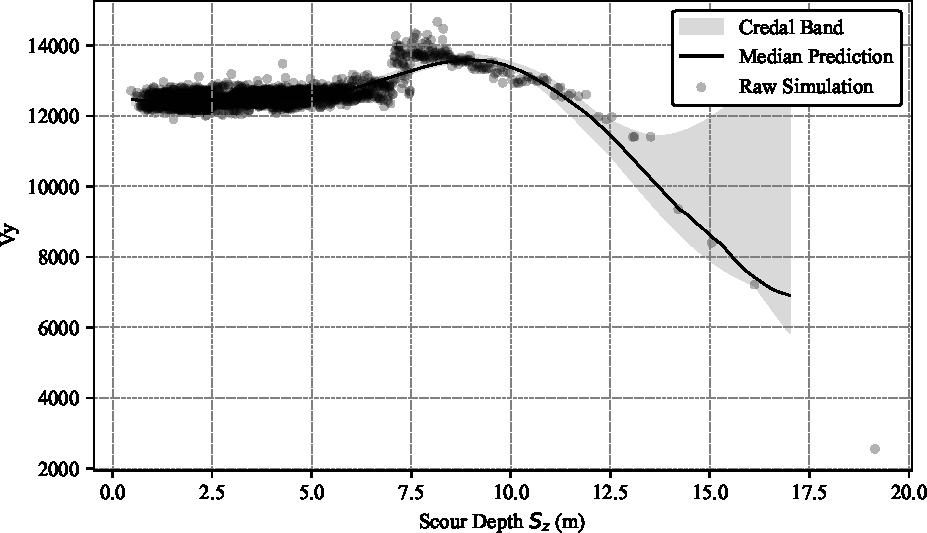
\includegraphics[width=\linewidth]{Figures/Figure08a.pdf}
        \caption{}
        \label{fig:figure8a}
\end{subfigure}
\hfill
     \begin{subfigure}[b]{0.48\textwidth}
        \centering
        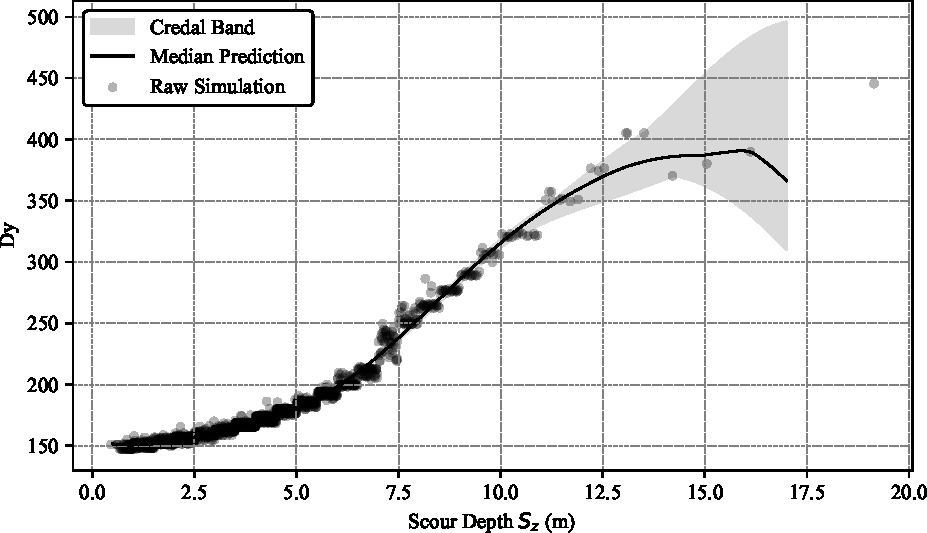
\includegraphics[width=\linewidth]{Figures/Figure08b.pdf}
        \caption{}
        \label{fig:figure8b}
\end{subfigure}
\hfill
     \begin{subfigure}[b]{0.48\textwidth}
        \centering
        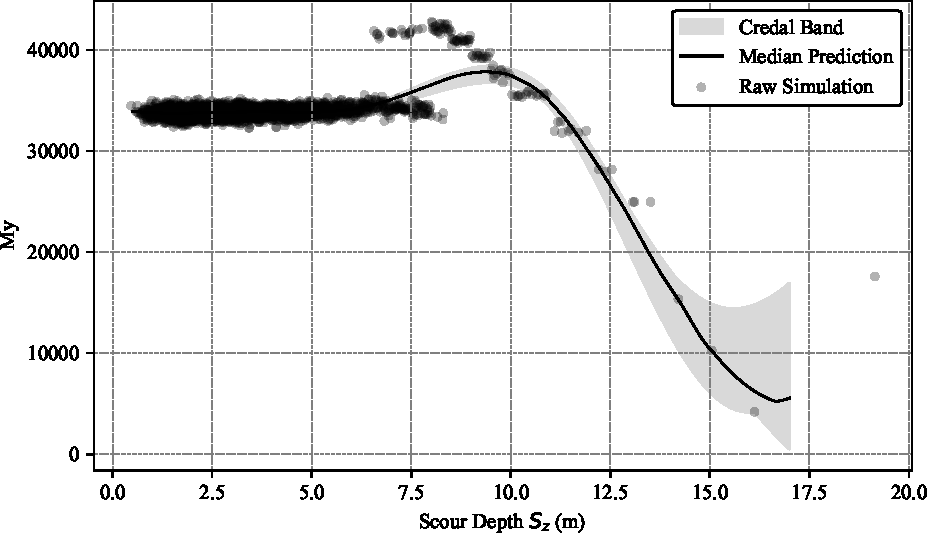
\includegraphics[width=\linewidth]{Figures/Figure08c.pdf}
        \caption{}
        \label{fig:figure8c}
\end{subfigure}
\hfill
     \begin{subfigure}[b]{0.48\textwidth}
        \centering
        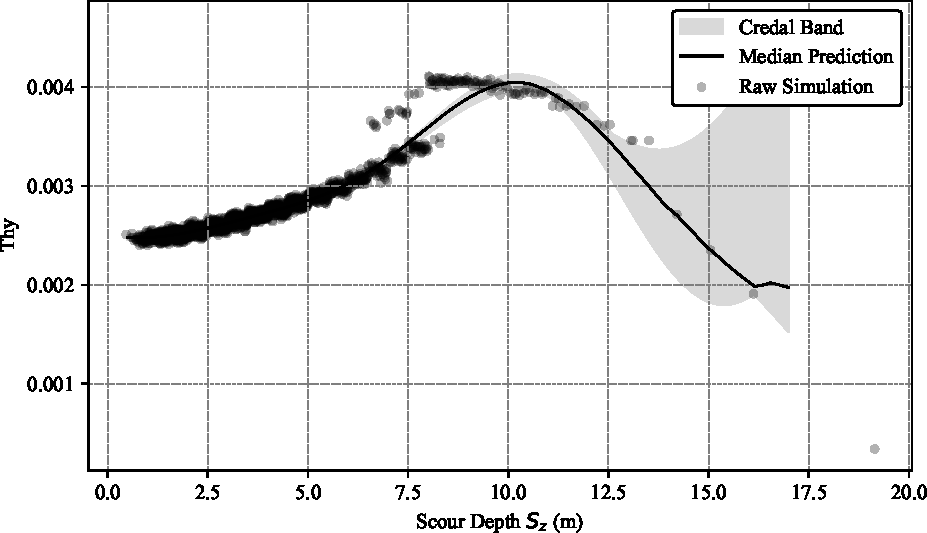
\includegraphics[width=\linewidth]{Figures/Figure08d.pdf}
        \caption{}
        \label{fig:figure8d}
\end{subfigure}
        \caption{Credal-set surrogate predictions using the SVR models compared against raw simulation data for yield capacities: (a) base shear ($V_y$), (b) deck displacement ($\Delta_y$), (c) base moment ($M_x$), and d-rotation ($\theta_x$) as functions of scour depth.} 
    \label{fig:figure8}
\end{figure}


\begin{figure}[htbp]
    \centering
     \begin{subfigure}[b]{0.48\textwidth}
        \centering
        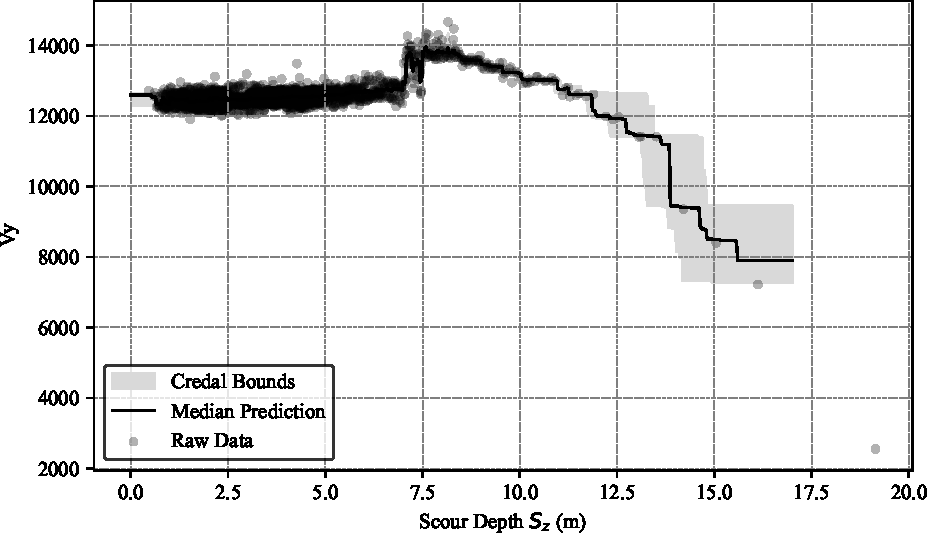
\includegraphics[width=\linewidth]{Figures/Figure09a.pdf}
        \caption{}
        \label{fig:figure9a}
\end{subfigure}
\hfill
     \begin{subfigure}[b]{0.48\textwidth}
        \centering
        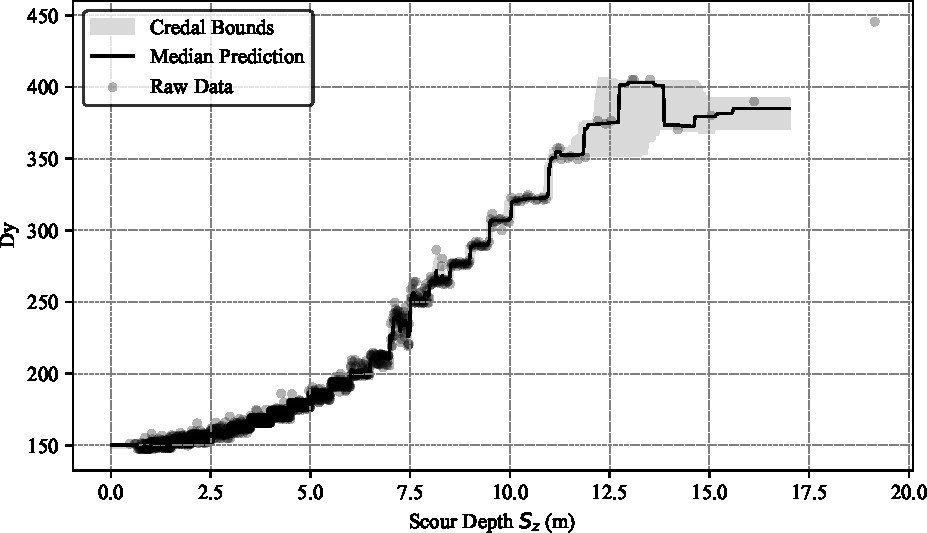
\includegraphics[width=\linewidth]{Figures/Figure09b.pdf}
        \caption{}
        \label{fig:figure9b}
\end{subfigure}
\hfill
     \begin{subfigure}[b]{0.48\textwidth}
        \centering
        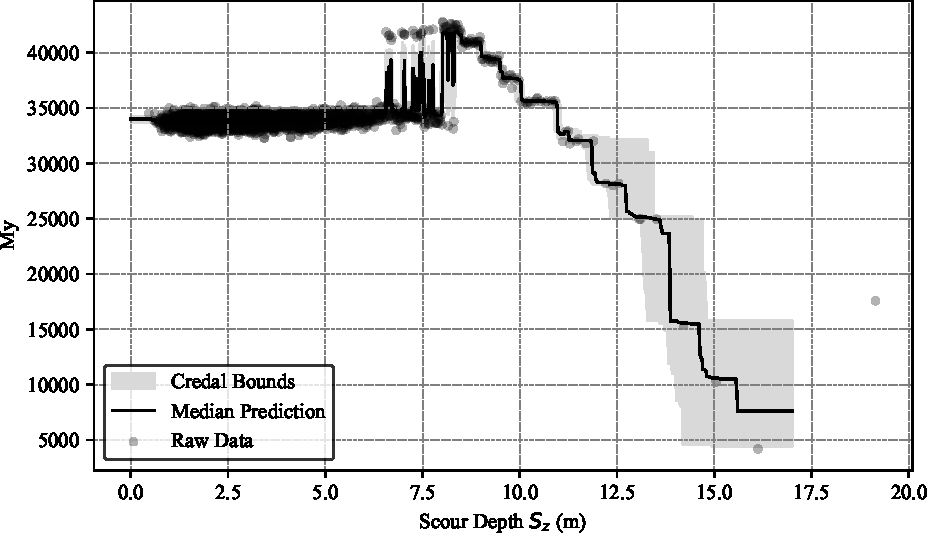
\includegraphics[width=\linewidth]{Figures/Figure09c.pdf}
        \caption{}
        \label{fig:figure9c}
\end{subfigure}
\hfill
     \begin{subfigure}[b]{0.48\textwidth}
        \centering
        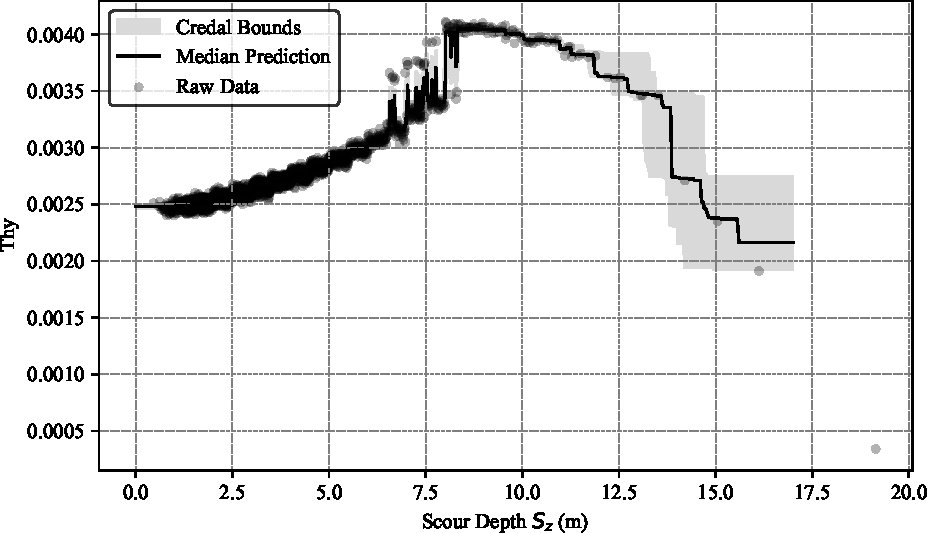
\includegraphics[width=\linewidth]{Figures/Figure09d.pdf}
        \caption{}
        \label{fig:figure9d}
\end{subfigure}
        \caption{Credal-set surrogate predictions using the GBR models compared against raw simulation data for yield capacities: (a) base shear ($V_y$), (b) deck displacement ($\Delta_y$), (c) base moment ($M_x$), and d-rotation ($\theta_x$) as functions of scour depth.} 
    \label{fig:figure9}
\end{figure}


\begin{table*}[htbp]
\caption{Credal-set Bounds for $\Delta_y$ and $V_y$ at Key Scour Depths}
\label{tab:credal_bounds}
\centering
\small
\begin{tabular}{|c|ccc||c|ccc|}
\hline
\multicolumn{4}{|c||}{\textit{GBR: Displacement $\Delta_y$ (mm)}} & \multicolumn{4}{c|}{\textit{SVR: Displacement $\Delta_y$ (mm)}} \\
\textit{Sz (mm)} & \textit{$C_{lb}$} & \textit{$C_{med}$} & \textit{$C_{ub}$} & \textit{Sz (mm)} & \textit{$C_{lb}$} & \textit{$C_{med}$} & \textit{$C_{ub}$} \\
\hline
500   & 148.78 & 149.85 & 150.37 & 500   & 164.76 & 198.47 & 236.69 \\
1000  & 148.64 & 149.44 & 151.68 & 1000  & 148.59 & 149.69 & 150.88 \\
5000  & 174.75 & 178.46 & 182.92 & 5000  & 181.25 & 181.51 & 181.87 \\
10000 & 305.90 & 307.51 & 321.04 & 10000 & 309.34 & 316.61 & 320.50 \\
15000 & 371.83 & 379.42 & 405.08 & 15000 & 272.62 & 378.04 & 383.41 \\
\hline
\multicolumn{4}{|c||}{\textit{GBR: Base Shear $V_y$ (kN)}} & \multicolumn{4}{c|}{\textit{SVR: Base Shear $V_y$ (kN)}} \\
\textit{Sz (mm)} & \textit{$C_{lb}$} & \textit{$C_{med}$} & \textit{$C_{ub}$} & \textit{Sz (mm)} & \textit{$C_{lb}$} & \textit{$C_{med}$} & \textit{$C_{ub}$} \\
\hline
500   & 12365.31 & 12444.08 & 12516.64 & 500   & 11257.10 & 13662.76 & 15388.41 \\
1000  & 12328.49 & 12420.52 & 12508.12 & 1000  & 12332.42 & 12366.90 & 12497.20 \\
5000  & 12311.38 & 12475.22 & 12592.03 & 5000  & 12582.51 & 12618.92 & 12639.30 \\
10000 & 13016.54 & 13159.33 & 13235.98 & 10000 & 13050.03 & 13133.21 & 13234.92 \\
15000 & 7346.25  & 8488.96  & 11497.43 & 15000 & 8313.01  & 8476.01  & 11400.96 \\
\hline
\end{tabular}
\normalsize
\end{table*}

These results indicate that both SVR and GBR effectively approximate the nonlinear relationship between scour depth and structural capacity. GBR performed better in capturing the capacity transitions when non-smooth and set-valued relations occur. SVR, using smooth RBF kernels, offered a good generalization but exhibited limitations in modeling those non-differentiable relations between the capacity and the scour depth.  The credal-set formulation effectively conveys epistemic uncertainty stemming from both model specification and data sparsity. Prediction intervals widen notably in poorly sampled regions (i.e., extreme scour), indicating reduced confidence and the need for conservative estimates in those regimes. 



\subsection{Feature Dominance Analysis}
To interpret surrogate behavior and identify which features most influenced capacity predictions, a feature dominance analysis was conducted for both SVR and GBR models. The results from both models were largely consistent (the exception is discussed later). Since the GBR-based interpretation proved more informative due to its superior surrogating performance, feature dominance results based on the GBR models are described below. 

Figures~\ref {fig:figure10a} to~\ref{fig:figure10d} display the GBR-based feature dominance results for each of the four capacity outputs. These plots illustrate the cumulative contribution of each input feature, where segment count represents the number of times a feature was selected as a decision-splitting node across all trees in the ensemble. A higher count indicates a greater influence on predictive decisions. Figure~\ref{fig:figure11a} to~\ref{fig:figure11d} visualizes the most dominant feature as the scour depth varies based on the GBR model as well. 

\begin{figure}[htbp]
    \centering
     \begin{subfigure}[b]{0.48\textwidth}
        \centering
        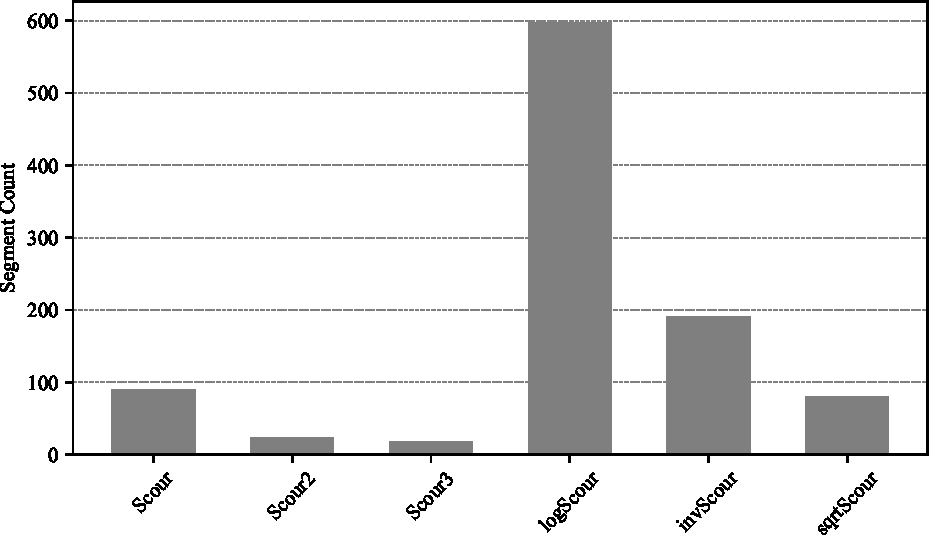
\includegraphics[width=\linewidth]{Figures/Figure10a.pdf}
        \caption{}
        \label{fig:figure10a}
\end{subfigure}
\hfill
     \begin{subfigure}[b]{0.48\textwidth}
        \centering
        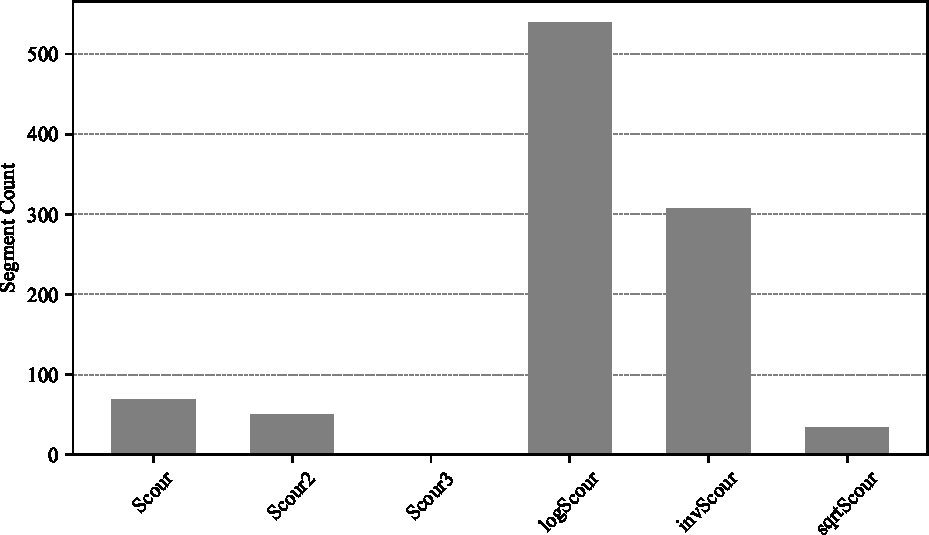
\includegraphics[width=\linewidth]{Figures/Figure10b.pdf}
        \caption{}
        \label{fig:figure10b}
\end{subfigure}
\hfill
     \begin{subfigure}[b]{0.48\textwidth}
        \centering
        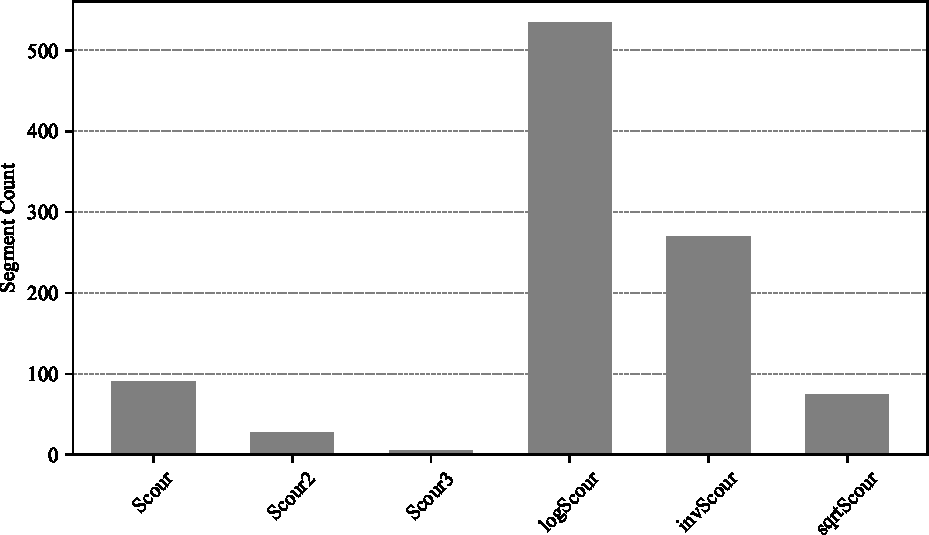
\includegraphics[width=\linewidth]{Figures/Figure10c.pdf}
        \caption{}
        \label{fig:figure10c}
\end{subfigure}
\hfill
     \begin{subfigure}[b]{0.48\textwidth}
        \centering
        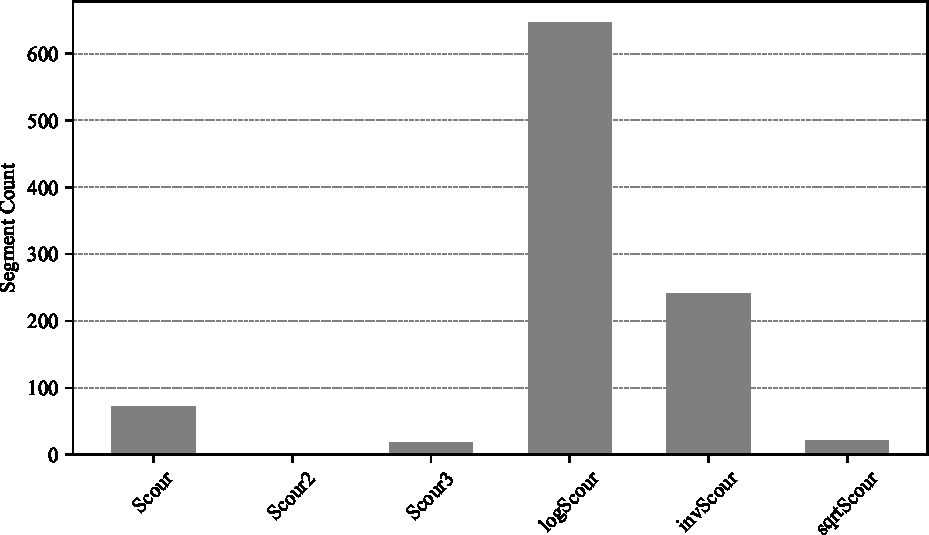
\includegraphics[width=\linewidth]{Figures/Figure10d.pdf}
        \caption{}
        \label{fig:figure10d}
\end{subfigure}
        \caption{Bar charts of feature dominance counts for each capacity measure, indicating the frequency with which each scour-derived input dominates predictions in the GBR surrogate models:  (a) $V_y$, (b) $\Delta_y$, (c) $M_x$, and (d) $\theta_x$. Note that the input features of \textit{Scour}, \textit{Scour2}, \textit{Scour3}, \textit{logScour},\textit{InvScour}, and \textit{sqrtScour}, representing $S_z$: $S_z^2$, $S_z^3$, $\log(S_z)$, $1/S_z$, and $\sqrt{S_z}$, respectively.} 
    \label{fig:figure10}
\end{figure}


\begin{figure}[htbp]
    \centering
     \begin{subfigure}[b]{0.48\textwidth}
        \centering
        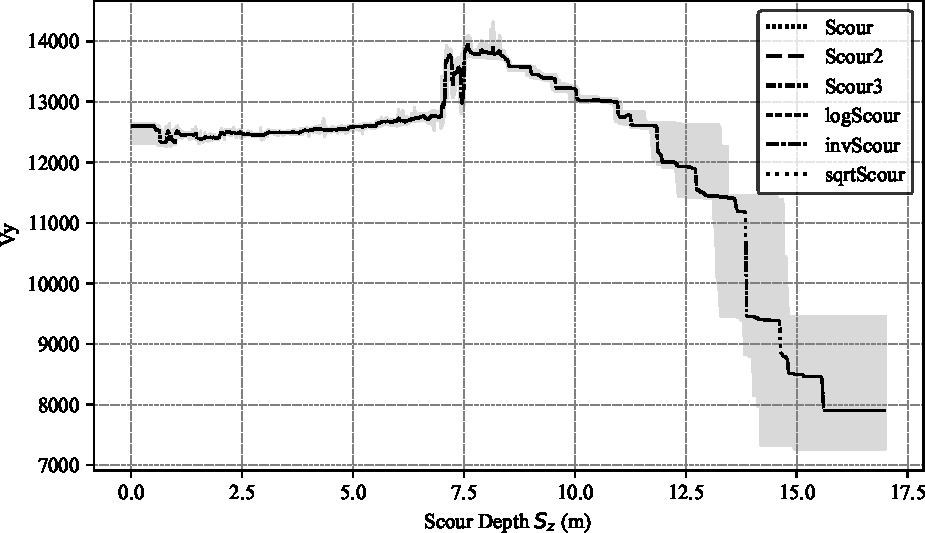
\includegraphics[width=\linewidth]{Figures/Figure11a.pdf}
        \caption{}
        \label{fig:figure11a}
\end{subfigure}
\hfill
     \begin{subfigure}[b]{0.48\textwidth}
        \centering
        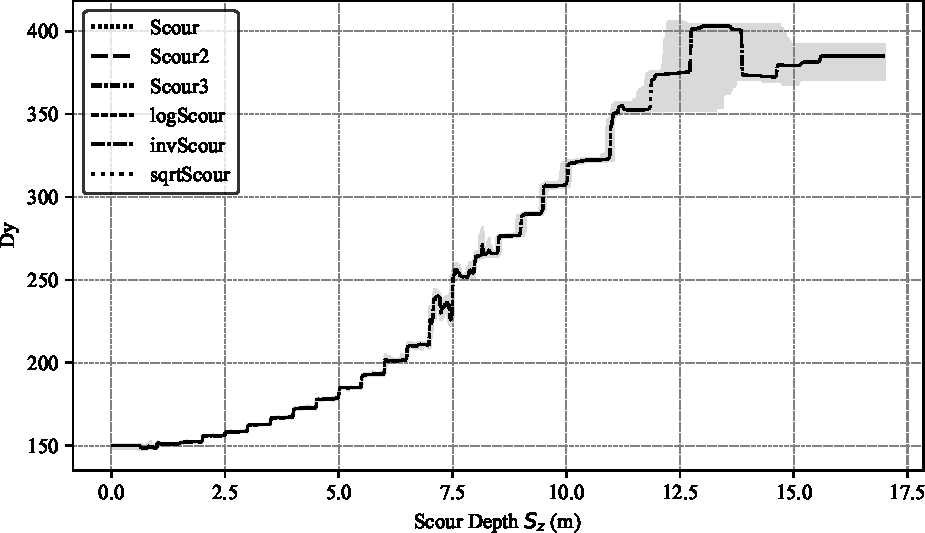
\includegraphics[width=\linewidth]{Figures/Figure11b.pdf}
        \caption{}
        \label{fig:figure11b}
\end{subfigure}
\hfill
     \begin{subfigure}[b]{0.48\textwidth}
        \centering
        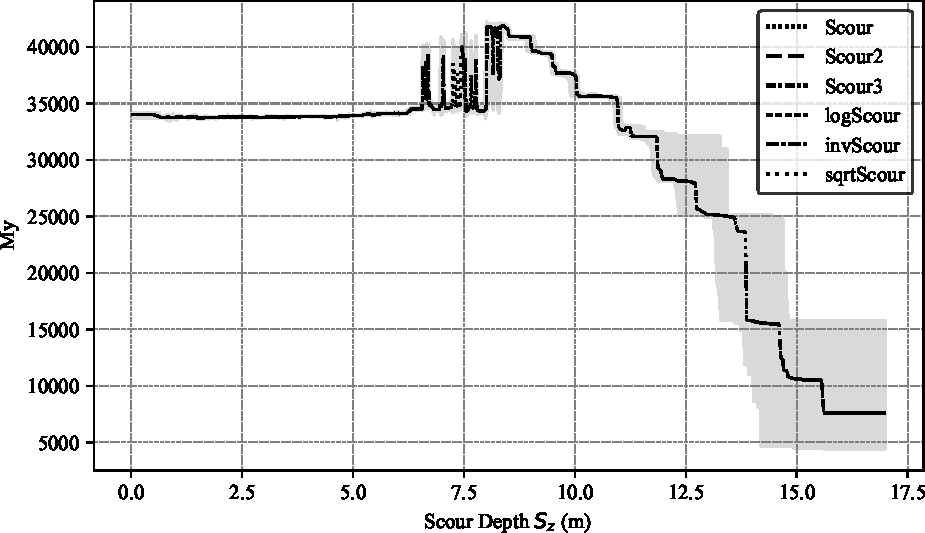
\includegraphics[width=\linewidth]{Figures/Figure11c.pdf}
        \caption{}
        \label{fig:figure11c}
\end{subfigure}
\hfill
     \begin{subfigure}[b]{0.48\textwidth}
        \centering
        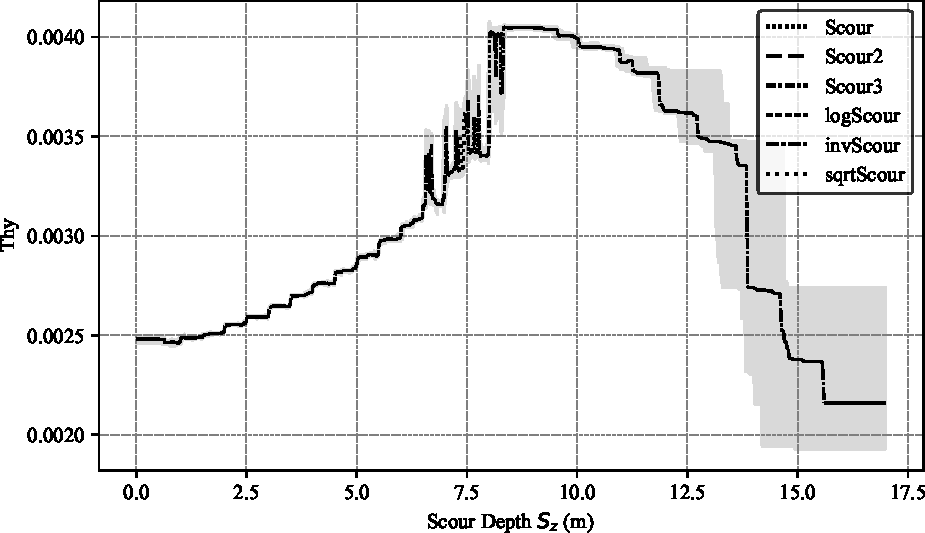
\includegraphics[width=\linewidth]{Figures/Figure11d.pdf}
        \caption{}
        \label{fig:figure11d}
\end{subfigure}
        \caption{Scour-depth varying visualization of most dominant features for target capacity based on the GBR surrogate models: (a) $V_y$, (b) $\Delta_y$, (c) $M_x$, and (d) $\theta_x$. Note that the input features of \textit{Scour}, \textit{Scour2}, \textit{Scour3}, \textit{logScour},\textit{InvScour}, and \textit{sqrtScour}, representing $S_z$: $S_z^2$, $S_z^3$, $\log(S_z)$, $1/S_z$, and $\sqrt{S_z}$, respectively.} 
    \label{fig:figure11}
\end{figure}

The analysis reveals that the logarithmic transformation of scour depth (\textit{logScour}) or  $\log(S_z)$, was the most dominant feature across all capacity components. Other engineered features such as inverse scour depth ($1/S_z$), square root of scour depth ($\sqrt{S_z}$), and quadratic terms ($S_z^2$) gained prominence, particularly at larger scour depths, where capacity responses exhibit asymptotic or nonlinear decline. These findings support the inclusion of a diverse set of engineered features to enhance surrogate model expressiveness across different scour regimes.



\section{Discussion}

The proposed surrogate modeling framework, integrated with credal-set uncertainty quantification, provides a computationally efficient and conservative approach for evaluating bridge capacity degradation under deep, climate-driven uncertainties. We highlight several limitations, practical implications, and directions for future work, as summarized below.

\begin{itemize}

    % \item \textit{Limitation 1: Scope of Uncertainty Representation.} In this work, scour is treated as the dominant source of uncertainty when considering climate scenarios. Material uncertainties (i.e., concrete compressive strength and steel yield strength) are subject to numerous environmental factors, many of which are affected by climate change. Such uncertainty propagation due to material properties and their compounding with scour depths is not considered.

\item \textit{Limitation 1: Scope of Uncertainty Representation.} 
In this work, scour is treated as the dominant causal source of uncertainty when assessing bridge capacity degradation under climate scenarios. Material uncertainties (i.e., concrete compressive strength and steel yield strength) were incorporated in the FE simulations as random variables but were treated as background fluctuations rather than causal drivers of scour effects. 
We recognize that, in a more comprehensive climate-change context, variables such as ambient temperature, moisture, and corrosion may lead to progressive material degradation and thus partially and causally affect bridge capacity. In such cases, a multi-input surrogate modeling framework that integrates both environmental and material factors would become essential for accurate and generalizable prediction. 



    \item \textit{Limitation 2: Surrogate Validity and Simulation Fidelity.} 
    Surrogate predictions inherently rely on the fidelity of the FE simulations used for training. Any model misspecification—such as in the soil–structure interaction formulation, boundary condition assumptions, or pier section modeling—may propagate variations into surrogate outcomes. In this work, we observed that non-smooth and set-valued nonlinearities occur when the scour depth reaches about $7.5\ \mathrm{m}$. The resulting nonlinear pushover curve becomes ‘unstable’ in manifesting the yielding points, leading to ‘jumped’ or ‘one-to-many’ localized relations. It is expected that by introducing additional or improved soil springs, such nonlinear behavior may be mitigated, thereby producing stable and more continuous extraction of capacity values. In this work, this is treated as a limitation in the fidelity of the physical system modeling process; nonetheless, it contributes to the epistemic uncertainties. Ultimately, while the surrogates show strong performance on simulated data, the practical deployment of the proposed methodology requires validation of the physical model against experimental, monitored, or field-assessed performance data.

    \item \textit{Implication 1: Importance of Feature Engineering.} 
    A notable insight is the central role of feature engineering in enhancing model performance. Both SVR and GBR consistently ranked transformed features—particularly $\log(S_z)$—as most influential. SVR emphasized $\log(S_z)$ and $\sqrt{S_z}$, aligning with its preference for smooth, kernel-based representations. In contrast, GBR favored $\log(S_z)$ and $1/S_z$, reflecting its strength in modeling sharp capacity transitions through decision-tree partitioning.

    \item \textit{Implication 2: Extensibility to Capacity–Demand Analysis.} 
    The current framework focuses on modeling intrinsic structural capacities under scour. However, understanding collapse vulnerability necessitates integrating extrinsic response demands, such as those from seismic loading or barge impacts. These demands are inherently stochastic and scenario-dependent. Future work should consider extending the surrogate approach to model both capacities and demands, enabling reliability-based assessment using credal-set formulations that avoid restrictive distributional assumptions.

    \item \textit{Practical Value and Future Extension.} 
    The use of surrogate learning and credal-set intervals to frame capacity prediction—namely, in terms of $(C_{lb}, C_{med}, C_{ub})$ rather than a single-valued prediction—offers an informed and interpretable framework for risk-informed decision-making. This is particularly relevant in resilience planning, where high-stakes infrastructure decisions must be made under poorly understood or evolving environmental conditions. Moving forward, integrating credal-based predictions into decision models that account for socioeconomic and behavioral factors (e.g., through multi-criteria or game-theoretic frameworks) represents an important avenue for interdisciplinary extension.

\end{itemize}

\section{Conclusion}

This study developed and demonstrated a surrogate-based framework for evaluating the yield-level capacity degradation of scour-critical bridges under deeply uncertain climate-driven scour scenarios. By integrating nonlinear pushover simulations with machine learning surrogates and credal-set uncertainty quantification, the framework enables both computational efficiency and distribution-agnostic capacity estimation.

Specifically, a suite of nonlinear finite-element analyses was conducted across 3,000 sampled scour conditions, generating a large-scale dataset of capacity responses. These responses were organized as a multi-dimensional capacity tuple (deck displacement, base shear, column moment, and rotation) at yield to characterize both superstructure and substructure performance. Two classes of surrogate models, Support Vector Regression (SVR) and Gradient Boosting Regression (GBR) were trained using both raw and engineered features of scour depth to emulate the simulation outputs. Feature engineering, especially logarithmic and inverse transformations of scour depth, was shown to be critical for capturing nonlinear capacity trends.

To address deep epistemic uncertainty associated with future scour severity, a credal-set formulation was employed using bootstrap ensembles. For each surrogate model, bootstrapped resamples were trained and evaluated, yielding lower and upper bounds on capacity predictions for any input scour depth. These credal bounds formed objective and distribution-agnostic intervals suitable for decision-making under high uncertainty. Comparative performance evaluation showed that GBR consistently outperformed SVR in prediction accuracy across all capacity metrics, while SVR provided smoother uncertainty envelopes in the scour-depth regime.

The results demonstrate that the proposed framework not only reduces computational cost but also explicitly accommodates structural and environmental uncertainty in a way that is practical and scalable. The methodology advances current practice by framing capacity prediction as an interval-based decision support tool and offers a path forward for risk-informed infrastructure assessment under progressive climate impacts.


\bibliographystyle{elsarticle-harv} 
\bibliography{references_updated}
\end{document}
